%% Baseado no arquivo: 
%% abtex2-modelo-trabalho-academico.tex, v-1.9.6 laurocesar
%% by abnTeX2 group at http://www.abntex.net.br/ 
%% Adaptado para um modelo dssse TCC (Graduação)

% ------------------------------------------------------------------------
% ------------------------------------------------------------------------
% abnTeX2: Modelo de Trabalho Academico (tese de doutorado, dissertacao de
% mestrado e trabalhos monograficos em geral) em conformidade com 
% ABNT NBR 14724:2011: Informacao e documentacao - Trabalhos academicos -
% Apresentacao
% ------------------------------------------------------------------------
% ------------------------------------------------------------------------

\documentclass[
	% -- opções da classe memoir --
	12pt,				% tamanho da fonte
	openright,			% capítulos começam em pág ímpar (insere página vazia caso preciso)
	oneside,			% para impressão em recto e verso. Oposto a oneside
	a4paper,			% tamanho do papel. 
	% -- opções da classe abntex2 --
	%chapter=TITLE,		% títulos de capítulos convertidos em letras maiúsculas
	%section=TITLE,		% títulos de seções convertidos em letras maiúsculas
	%subsection=TITLE,	% títulos de subseções convertidos em letras maiúsculas
	%subsubsection=TITLE,% títulos de subsubseções convertidos em letras maiúsculas
	% -- opções do pacote babel --
	english,			% idioma adicional para hifenização
	%french,				% idioma adicional para hifenização
	%spanish,			% idioma adicional para hifenização
	brazil				% o último idioma é o principal do documento
	]{abntex2}

% ---
% Pacotes básicos 
% ---
\usepackage{lmodern}			% Usa a fonte Latin Modern			
\usepackage[T1]{fontenc}		% Selecao de codigos de fonte.
\usepackage[utf8]{inputenc}		% Codificacao do documento (conversão automática dos acentos)
\usepackage{lastpage}			% Usado pela Ficha catalográfica
\usepackage{indentfirst}		% Indenta o primeiro parágrafo de cada seção.
\usepackage{color}				% Controle das cores
\usepackage{graphicx}			% Inclusão de gráficos
\usepackage{microtype} 			% para melhorias de justificação
\usepackage{float}				% para controle de posicionamento de figuras e tabelas
\usepackage{pdfpages} 			% para inclusão de PDFs
\usepackage{breqn}              % para quebrar equações
% ---
		

% ---
% Pacotes de citações
% ---
\usepackage[brazilian,hyperpageref]{backref}	 % Paginas com as citações na bibl
\usepackage[alf, bibjustif]{abntex2cite}	% Citações padrão ABNT

% --- 
% CONFIGURAÇÕES DE PACOTES
% --- 

% ---
% Configurações do pacote backref
% Usado sem a opção hyperpageref de backref
\renewcommand{\backrefpagesname}{%Citado na(s) página(s):~
}
% Texto padrão antes do número das páginas
\renewcommand{\backref}{}
% Define os textos da citação
\renewcommand*{\backrefalt}[4]{
	%\ifcase #1 %
	%	Nenhuma citação no texto.%
	%\or
	%	Citado na página #2.%
	%\else
	%	Citado #1 vezes nas páginas #2.%
	%\fi
    }%
% ---

% ---
% Informações de dados para CAPA e FOLHA DE ROSTO
% ---
\titulo{Jogo de Xadrez com Manipuladores Robóticos}
\autor{Rafael Dias Campos}
\local{Belo Horizonte}
\data{2023}
\orientador{Ramon da Cunha Lopes}
\instituicao{%
  Centro Federal de Educação Tecnológica de Minas Gerais -- CEFET-MG
  \par
  Departamento de Computação
  \par
  Curso de Engenharia da Computação
  }
\tipotrabalho{Monografia (Graduação)}
% O preambulo deve conter o tipo do trabalho, o objetivo, 
% o nome da instituição e a área de concentração 
\preambulo{Trabalho de Conclusão de Curso apresentado ao Curso
de Engenharia de Computação do Centro Federal de
Educação Tecnológica de Minas Gerais, como requisito
parcial para a obtenção do título de Bacharel em
Engenharia de Computação.}
% ---


% ---
% Configurações de aparência do PDF final

% alterando o aspecto da cor azul
\definecolor{blue}{RGB}{41,5,195}

% informações do PDF
\makeatletter
\hypersetup{
     	%pagebackref=true,
		pdftitle={\@title}, 
		pdfauthor={\@author},
    	pdfsubject={\imprimirpreambulo},
	    pdfcreator={LaTeX with abnTeX2},
		pdfkeywords={abnt}{latex}{abntex}{abntex2}{trabalho acadêmico}, 
		colorlinks=true,       		% false: boxed links; true: colored links
		% hidelinks=true,
    	linkcolor=blue,          	% color of internal links
    	citecolor=blue,        		% color of links to bibliography
    	filecolor=magenta,      		% color of file links
		urlcolor=blue,
		bookmarksdepth=4
}
\makeatother
% --- 

% --- 
% Espaçamentos entre linhas e parágrafos 
% --- 

% O tamanho do parágrafo é dado por:
\setlength{\parindent}{1.3cm}

% Controle do espaçamento entre um parágrafo e outro:
\setlength{\parskip}{0.2cm}  % tente também \onelineskip

% ---
% compila o indice
% ---
\makeindex
% ---

% ----
% Início do documento
% ----
\begin{document}

% Seleciona o idioma do documento (conforme pacotes do babel)
%\selectlanguage{english}
%\selectlanguage{brazil}

% Retira espaço extra obsoleto entre as frases.
\frenchspacing 

% ----------------------------------------------------------
% ELEMENTOS PRÉ-TEXTUAIS
% ----------------------------------------------------------



%% Baseado no arquivo: 
%% abtex2-modelo-trabalho-academico.tex, v-1.9.6 laurocesar
%% by abnTeX2 group at http://www.abntex.net.br/ 
%% Adaptado para um modelo de TCC (Graduação)

% ---
% Capa
% ---
\imprimircapa
% ---

% ---
% Folha de rosto
% (o * indica que haverá a ficha bibliográfica)
% ---
\imprimirfolhaderosto*
% ---

% ---
% Inserir a ficha bibliografica
% ---

% Isto é um exemplo de Ficha Catalográfica, ou ``Dados internacionais de
% catalogação-na-publicação''. Você pode utilizar este modelo como referência. 
% Porém, provavelmente a biblioteca da sua universidade lhe fornecerá um PDF
% com a ficha catalográfica definitiva após a defesa do trabalho. Quando estiver
% com o documento, salve-o como PDF no diretório do seu projeto e substitua todo
% o conteúdo de implementação deste arquivo pelo comando abaixo:
%
% \begin{fichacatalografica}
%     
% \end{fichacatalografica}

\begin{fichacatalografica}
~
%\includepdf{fig_ficha_catalografica.pdf}
% 	\sffamily
% 	\vspace*{\fill}					% Posição vertical
% 	\begin{center}					% Minipage Centralizado
% 	\fbox{\begin{minipage}[c][8cm]{13.5cm}		% Largura
% 	\small
% 	\imprimirautor
% 	%Sobrenome, Nome do autor
	
% 	\hspace{0.5cm} \imprimirtitulo  / \imprimirautor. --
% 	\imprimirlocal, \imprimirdata-
	
% 	\hspace{0.5cm} \pageref{LastPage} p. : il. (algumas color.) ; 30 cm.\\
	
% 	\hspace{0.5cm} \imprimirorientadorRotulo~\imprimirorientador\\
	
% 	\hspace{0.5cm}
% 	\parbox[t]{\textwidth}{\imprimirtipotrabalho~--~\imprimirinstituicao,
% 	\imprimirdata.}\\
	
% 	\hspace{0.5cm}
% 		1. Palavra-chave1.
% 		2. Palavra-chave2.
% 		2. Palavra-chave3.
% 		I. Orientador.
% 		II. Universidade xxx.
% 		III. Faculdade de xxx.
% 		IV. Título 			
% 	\end{minipage}}
% 	\end{center}
\end{fichacatalografica}
% ---

% % ---
% % Inserir errata
% % ---
% \begin{errata}
% Elemento opcional da \citeonline[4.2.1.2]{NBR14724:2011}. Exemplo:

% \vspace{\onelineskip}

% FERRIGNO, C. R. A. \textbf{Tratamento de neoplasias ósseas apendiculares com
% reimplantação de enxerto ósseo autólogo autoclavado associado ao plasma
% rico em plaquetas}: estudo crítico na cirurgia de preservação de membro em
% cães. 2011. 128 f. Tese (Livre-Docência) - Faculdade de Medicina Veterinária e
% Zootecnia, Universidade de São Paulo, São Paulo, 2011.

% \begin{table}[htb]
% \center
% \footnotesize
% \begin{tabular}{|p{1.4cm}|p{1cm}|p{3cm}|p{3cm}|}
%   \hline
%    \textbf{Folha} & \textbf{Linha}  & \textbf{Onde se lê}  & \textbf{Leia-se}  \\
%     \hline
%     1 & 10 & auto-conclavo & autoconclavo\\
%    \hline
% \end{tabular}
% \end{table}

% \end{errata}
% ---

% ---
% Inserir folha de aprovação
% ---


%
\begin{folhadeaprovacao}

  \begin{center}
    Espaço destinado à folha de aprovação
%após aprovação, insira a cópia da folha de aprovação por meio do comando:
% \includepdf{folhadeaprovacao_final.pdf}
  \end{center}
  
\end{folhadeaprovacao}
% ---

% ---
% Dedicatória
% ---
\begin{dedicatoria}
   \vspace*{\fill}
   \centering
   \noindent
   \textit{Dedico este trabalho aos alunos(as) do CEFET-MG.} \vspace*{\fill}
\end{dedicatoria}
% ---

% ---
% Agradecimentos
% ---
\begin{agradecimentos}
Agradeço ao Latex e às pessoas que contribuiram com o desenvolvimento do Abntex2 por facilitarem a vida dos graduandos.
\end{agradecimentos}
% ---

% ---
% Epígrafe
% ---
\begin{epigrafe}
    \vspace*{\fill}
	\begin{flushright}
		\textit{``As pessoas costumam dizer que a motivação não dura sempre. Bem, nem o efeito do banho, por isso recomenda-se diariamente.''\\
		(Zig Ziglar)}
	\end{flushright}
\end{epigrafe}
% ---

% ---
% RESUMOS
% ---

% resumo em português
\setlength{\absparsep}{18pt} % ajusta o espaçamento dos parágrafos do resumo
\begin{resumo}
Neste trabalho será realizado o controle digital de dois manipuladores robóticos para a movimentação de peças de Xadrez. 

Inicialmente, será realizado o controle de um manipulador para possibilitar que um ser-humano jogue uma partida com o computador.
Em seguida, o segundo manipulador será controlado para que duas pessoas joguem uma partida entre si.

 \textbf{Palavras-chave}: Manipuladores Robóticos. Controle Digital. Xadrez
\end{resumo}

% resumo em inglês
\begin{resumo}[Abstract]
 \begin{otherlanguage*}{english}
   In this thesis, will be implemented the digital control of two robotic arms to move chess pieces.

   Initially, a single arm will be controlled in order to allow a human player to play against the computer.
   Further on, the second arm will be controlled so that two human players can play against each other.

   \vspace{\onelineskip}
 
   \noindent 
   \textbf{Keywords}: Robotic Arms. Digital Control. Chess.
 \end{otherlanguage*}
\end{resumo}


% ---

% ---
% inserir lista de ilustrações
% ---
\pdfbookmark[0]{\listfigurename}{lof}
\listoffigures*
\cleardoublepage
% ---

% ---
% inserir lista de tabelas
% ---
\pdfbookmark[0]{\listtablename}{lot}
\listoftables*
\cleardoublepage
% ---

% ---
% inserir lista de abreviaturas e siglas
% ---
\begin{siglas}
  \item[CEFET-MG] Centro Federal de Educação Tecnológica de Minas Gerais
  \item[STEM] \textit{Science, Technology, Engineering and Mathematics} [Ciência, Tecnologia, Engenharia e Matemática]
\end{siglas}
% ---

% ---
% inserir lista de símbolos
% ---
\begin{simbolos}
  \item[$ \Gamma $] Letra grega Gama
  \item[$ \Lambda $] Lambda
  \item[$ \zeta $] Letra grega minúscula zeta
  \item[$ \in $] Pertence
\end{simbolos}
% ---

% ---
% inserir o sumario
% ---
\pdfbookmark[0]{\contentsname}{toc}
\tableofcontents*
\cleardoublepage
% ---

% ----------------------------------------------------------
% ELEMENTOS TEXTUAIS
% ----------------------------------------------------------
\textual

% ----------------------------------------------------------
% Como o documento será grande, sugiro dividir em diversos arquivos, um para cada capítulo.
% ----------------------------------------------------------


\chapter[Introdução]{Introdução}
\label{cap:introducao}

Atualmente, existe uma grande procura por funcionários especializados em Tecnologia da Informação (TI) e áreas similares,
sendo percebida no mundo todo uma grande carência de profissionais qualificados para atuar nessas áreas \cite{shortage_of_workers}.

Com base nisso, foi proposto realizar o desenvolvimento de uma plataforma que utilize recursos computacionais passível de ser utilizada para demonstrar conceitos nas áreas de computação, elétrica e controle.
Para aumentar o interesse por ela foi definido que deve permitir que os participantes joguem uma partida de Xadrez.

Correlacionando essas ideias, foi decidido implementar um jogo de Xadrez que pode ser jogado através de braços robóticos.

\section[Motivação]{Motivação}

Considerando a carência de profissionais de TI no mercado, torna-se importante a busca por formas de incentivar o aprendizado e a busca por conhecimento por parte dos jovens.
Para tornar o aprendizado mais atrativo e divertido, foi feita a incorporação de um jogo no projeto proposto.
Finalmente, foi decidido que o projeto deveria usar elementos da robótica, visto que pesquisas demonstram que seu uso em atividades com crianças consegue influenciar positivamente o desenvolvimento de habilidades da área de STEM \cite{technology_for_stem}.

\section[Objetivos]{Objetivos}

Este trabalho visa desenvolver um sistema de controle de manipuladores robóticos que permitam que dois jogadores participem em uma partida de Xadrez.

Caso haja disponibilidade de tempo, o sistema também possibilitará que o jogo seja jogado por um jogador humano e um computador ou jogador humano através da Internet.

\section[Relevância]{Relevância}

Com o desenvolvimento dessa plataforma, será possível demonstrar conceitos de computação, elétrica e controle de forma prática e divertida.
Ela pode ser facilmente transportada para diferentes locais e apresentada em eventos, como feiras de ciências, por exemplo.
Dessa forma, ela pode promover e instigar a busca por conhecimento, além de atrair futuros profissionais para a área de TI.

\chapter[Trabalhos Relacionados]{Trabalhos Relacionados}
\label{cap:trabalhosRelacionados}

Durante a pesquisa realizada para o desenvolvimento deste trabalho, foram encontrados alguns trabalhos que apresentam características semelhantes ao que foi proposto.
Neste capítulo, serão apresentados alguns desses trabalhos, para mostrar o que foi feito e como foi feito, além de mostrar as diferenças entre eles e o trabalho proposto.

O trabalho apresentado por \citeauthor{jogador_xadrez} (\citeyear{jogador_xadrez}) apresenta um sistema para jogar xadrez contra um computador utilizando um tabuleiro físico.
Neste trabalho, foi desenvolvido um tabuleiro modificado que utiliza motores de passo e um eletroímã para movimentar as peças, conforme apresentado na Figura \ref{fig:jogadorXadrez}.
Além disso, foi implementado um sistema de visão computacional para detectar qual peça foi movimentada pelo jogador.

\begin{figure}[H]
    \centering
    \caption{Jogador de Xadrez Robótico com Visão Computacional}
    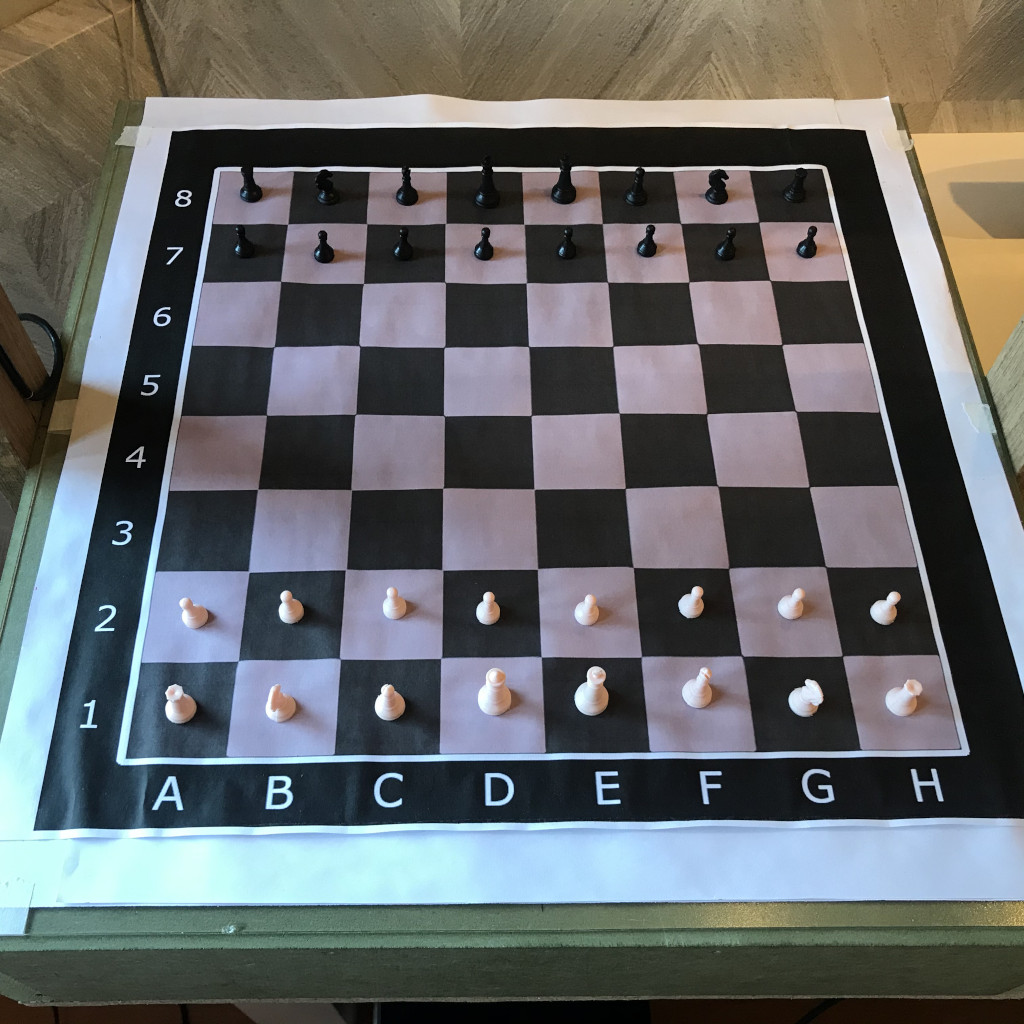
\includegraphics[keepaspectratio=true, width=0.6\textwidth]
    	{img/jogador-xadrez.jpg}
    \fonte{\citeauthor{jogador_xadrez} (\citeyear{jogador_xadrez})}
    \label{fig:jogadorXadrez}
\end{figure}

Em outra frente, o trabalho de \citeauthor{ferramenta_braco_robotico} (\citeyear{ferramenta_braco_robotico}) apresenta uma ferramenta para manipular um braço robótico utilizando um computador.
Essa ferramenta recebe os ângulos desejados de cada junta do braço e realiza o movimento, utilizando-se de cinemática direta, conforme apresentado na Figura \ref{fig:ferramentaComputacional}.
Lançando-se mão dessa ferramenta, é possível movimentar o braço robótico com base nos ângulos,
entretanto não é possível diretamente definir sua posição final.

\begin{figure}[H]
    \centering
    \caption{Uma Ferramenta Computacional para Manipulação de um Braço Robótico}
    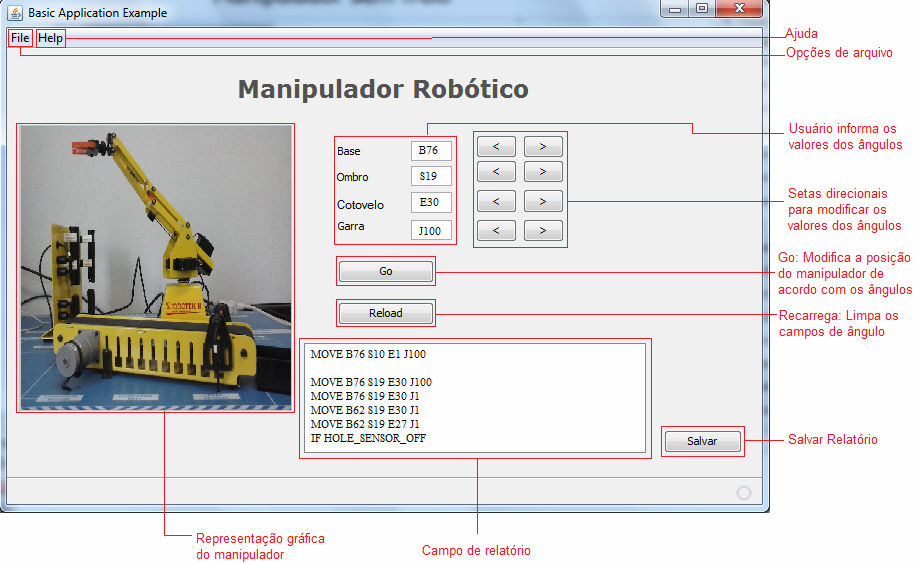
\includegraphics[keepaspectratio=true, width=0.95\textwidth]
    	{img/ferramenta-computacional.jpg}
    \fonte{\citeauthor{ferramenta_braco_robotico} (\citeyear{ferramenta_braco_robotico})}
    \label{fig:ferramentaComputacional}
\end{figure}

\citeauthor{inverse_kinematics_five_joint} (\citeyear{inverse_kinematics_five_joint}) apresenta um estudo sobre cinemática inversa de um braço robótico de cinco juntas.
Neste trabalho, é apresentado um método para calcular os ângulos de cada junta, com base na posição final desejada.
A partir desse método, é possível movimentar o braço robótico com mais facilidade, pois não é necessário calcular os ângulos manualmente.

A partir do estudo desses trabalhos, foi possível definir o escopo do trabalho proposto e observar as diferenças em relação aos trabalhos relacionados.
O trabalho proposto implementa o jogo de xadrez, assim como o trabalho de \citeauthor{jogador_xadrez} (\citeyear{jogador_xadrez}), porém utiliza um braço robótico para movimentar as peças.
Para isso, foi necessário desenvolver uma ferramenta que permite a comunicação entre um computador e o braço robótico, assim como o trabalho de \citeauthor{ferramenta_braco_robotico} (\citeyear{ferramenta_braco_robotico}). 
Por sua vez, o controle do braço é feito através de um sistema de cinemática inversa, assim como o trabalho de \citeauthor{inverse_kinematics_five_joint} (\citeyear{inverse_kinematics_five_joint}), porém com um menor número de juntas.

\chapter[Metodologia]{Metodologia}
\label{cap:metodologia}

O desenvolvimento do projeto foi dividido em duas etapas: uma de planejamento e outra de execução.

Durante a etapa de planejamento, foram definidos os componentes necessários para a construção do projeto, bem como a forma de integração entre eles.
Além disso, foi feito um estudo sobre o controle de um braço robótico e sobre as capacidades do microcontrolador escolhido para o projeto.

Na etapa de execução, foi feita primeiramente a montagem dos componentes físicos do projeto.
Em seguida, foi desenvolvido o \textit{software} do microcontrolador, que é responsável por controlar os motores e receber os comandos do usuário.
Por fim, foi desenvolvido o \textit{software} do computador para implementar as regras do jogo de xadrez e comunicar com o microcontrolador.

\chapter[Planejamento]{Planejamento}
\label{cap:planejamento}

Antes de iniciar o desenvolvimento do projeto, foi feita uma pesquisa sobre as regras do jogo de xadrez.
Em seguida, foram especificados os recursos necessários para a montagem do sistema e sua utilização.
Esta seção descreve as regras do jogo, a escolha do equipamento e o projeto inicial do sistema.

\section[Regras de xadrez]{Regras de xadrez}
\label{sec:xadrezRegras}

O jogo de xadrez é um jogo de tabuleiro para dois jogadores.
Sua origem é incerta, mas acredita-se que ele tenha surgido na Índia, antes mesmo da era cristã \cite{xadrez_historia}.

\subsection[Tabuleiro]{Tabuleiro}
\label{sub:xadrezTabuleiro}

O tabuleiro de xadrez é composto por 64 casas quadradas, alternadamente claras e escuras, dispostas em uma grade 8x8 conforme a Figura \ref{fig:xadrezTabuleiro}.
Cada casa é identificada por uma letra de \textit{a} a \textit{h} e um número de \textit{1} a \textit{8}
e pode comportar no máximo uma peça.

\begin{figure}[H]
    \centering
    \caption{Tabuleiro de xadrez}
    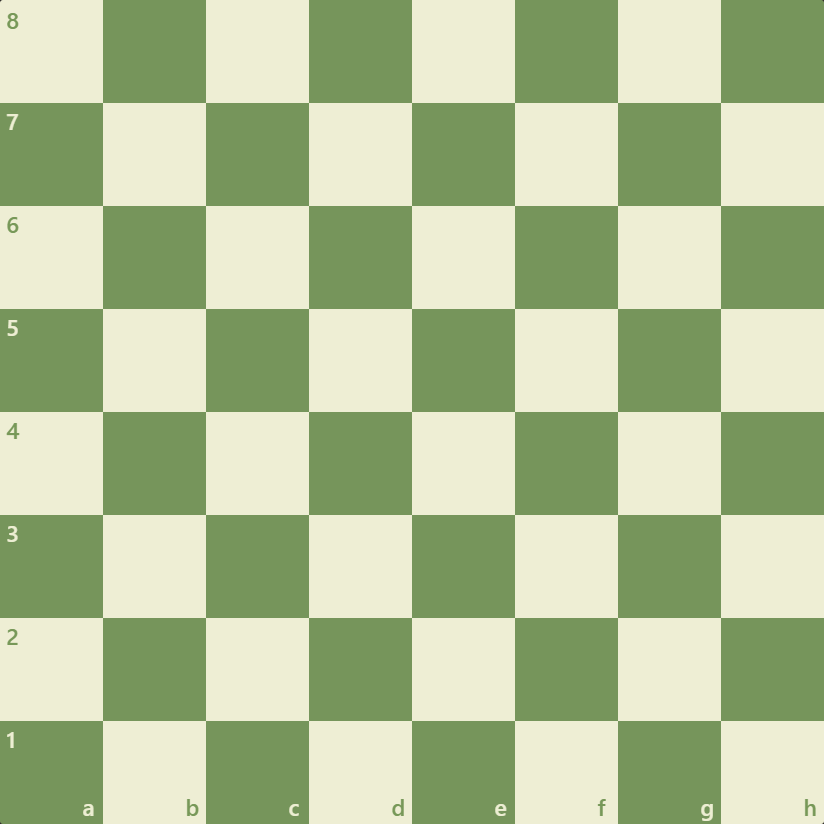
\includegraphics[keepaspectratio=true, width=0.6\textwidth]
    	{img/xadrez-tabuleiro.png}
    \fonte{\url{https://www.chess.com}}
    \label{fig:xadrezTabuleiro}
\end{figure}

\subsection[Peças]{Peças}
\label{sub:xadrezPecas}

O jogo de xadrez possui 6 tipos de peças ilustradas na Figura \ref{fig:xadrezPecas}.
Cada uma dessas peças utiliza diferentes regras para se movimentar pelo tabuleiro.

\begin{figure}[H]
    \centering
    \caption{Peças de xadrez}
    
\includegraphics[keepaspectratio=true, width=0.6\textwidth]
    	{img/xadrez-pecas.png}
    \fonte{Do próprio autor}
    \label{fig:xadrezPecas}
\end{figure}

O Rei é a peça mais importante do jogo, e pode se mover para qualquer casa adjacente, horizontal, vertical ou diagonalmente.
Entretanto, ele não pode se mover para uma casa em que esteja em xeque, ou seja, em que ele possa ser capturado na próxima jogada.

A Torre pode se mover para qualquer casa na mesma linha ou coluna em que se encontra.
Por outro lado, o Bispo pode se mover para qualquer casa na mesma diagonal em que se encontra.

A Dama é a peça mais poderosa do jogo, e pode se mover como um Bispo ou como uma Torre,
ou seja, ela pode se deslocar para qualquer casa na mesma linha, coluna ou diagonal em que se encontra.

O Cavalo pode se mover duas casas em uma direção e uma casa em uma direção perpendicular, em forma de um \textit{L}.
Ele também é a única peça que pode pular outras peças.

Por fim, o Peão pode se mover uma casa para frente, ou duas casas para frente se ainda não tiver se movido no jogo.
Ele também pode capturar uma peça adversária que esteja uma casa na diagonal à sua frente.

\subsection[Início do jogo]{Início do jogo}
\label{sub:xadrezInicioJogo}

Para se iniciar uma partida de xadrez, o tabuleiro deve ser posicionado de forma que a casa \textit{a1} seja branca.
As peças brancas devem ser posicionadas na primeira linha,
seguindo a ordem: Torre, Cavalo, Bispo, Dama, Rei, Bispo, Cavalo e Torre.
As peças pretas devem ser posicionadas na oitava linha, seguindo a mesma ordem.
Os peões brancos devem ser posicionados na segunda linha e os peões pretos na sétima linha.
A Figura \ref{fig:xadrezTabuleiroMontado} apresenta o tabuleiro no início de uma partida.

\begin{figure}[H]
    \centering
    \caption{Tabuleiro de xadrez no início de uma partida}
    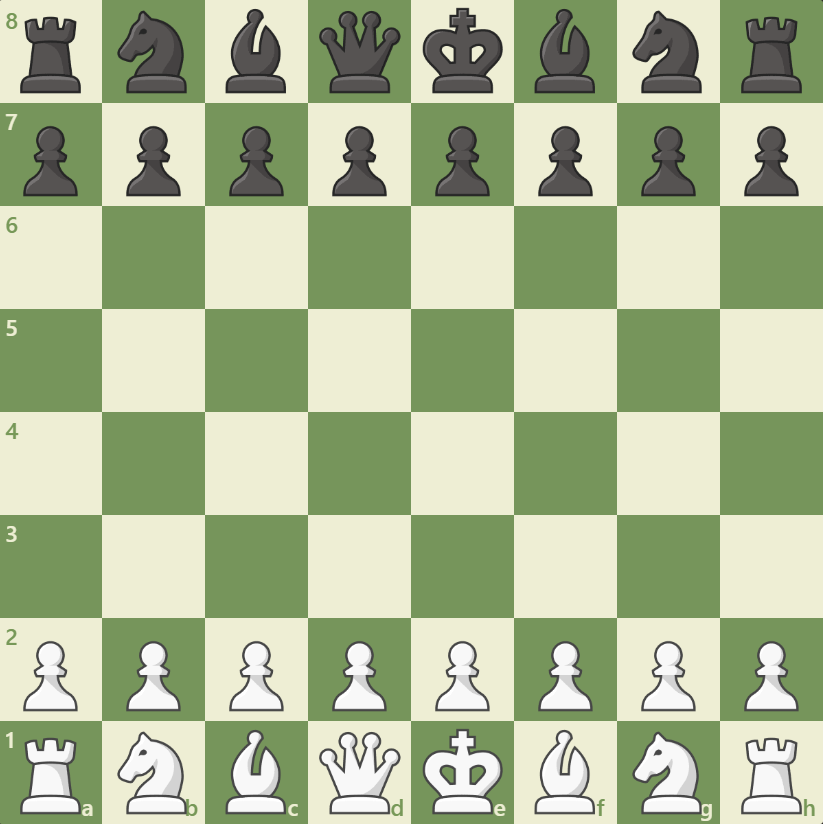
\includegraphics[keepaspectratio=true, width=0.6\textwidth]
    	{img/xadrez-tabuleiro-montado.png}
    \fonte{\url{https://www.chess.com}}
    \label{fig:xadrezTabuleiroMontado}
\end{figure}

Depois de montado o tabuleiro, o jogador que estiver com as peças brancas deve realizar a primeira jogada.
Em seguida, os jogadores devem realizar jogadas alternadas, até que o jogo termine conforme descrito na Subseção \ref{sub:xadrezFimJogo}.

\subsection[Fim de Jogo]{Fim de Jogo}
\label{sub:xadrezFimJogo}

O objetivo do jogo de xadrez é dar xeque-mate no Rei adversário, ou seja, deixar o Rei adversário em xeque e sem nenhuma casa para onde se mover.
Quando isso acontece, o jogo termina e o jogador que deu xeque-mate vence a partida.

Além disso, o jogo também pode terminar empatado.
Isso pode acontecer quando algum dos jogadores não possui nenhum movimento válido,
quando os jogadores concordam com o empate, quando o mesmo movimento é repetido três vezes
ou quando nenhum jogador tiver peças suficientes para dar xeque-mate.

\subsection[Movimentos especiais]{Movimentos especiais}

Além dos movimentos descritos na Subseção \ref{sub:xadrezPecas}, o jogo de xadrez possui alguns movimentos especiais.

O movimento de \textit{Roque} pode ser realizado pelo Rei e por uma Torre,
desde que ambas as peças ainda não tenham se movido no jogo e não haja nenhuma peça entre elas.
Para realizar o movimento, o Rei deve se mover duas casas em direção à Torre, e a Torre deve ser posicionada na casa adjacente ao Rei.
O movimento de \textit{Roque} pode ser realizado para a direita ou para a esquerda,
denominados \textit{Roque} curto e \textit{Roque} longo, com base na quantidade de casas que a Torre se move.

O movimento de \textit{En Passant} pode ser realizado por um Peão para capturar um Peão adversário em uma situação especial.
Caso o Peão adversário tenha se movido duas casas na jogada anterior, e esteja na mesma linha que um Peão capturador, é possível realizar o movimento de \textit{En Passant}.
Nesse caso, o Peão capturador deve se mover para a casa em que o Peão adversário estaria se tivesse se movido apenas uma casa na jogada anterior,
conforme ilustrado na Figura \ref{fig:xadrezEnPassant}.

\begin{figure}[H]
    \centering
    \caption{Movimento de \textit{En Passant}}
    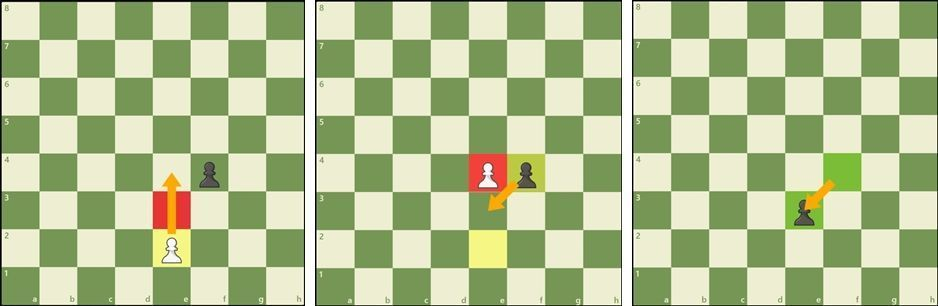
\includegraphics[keepaspectratio=true, width=0.9\textwidth]
    	{img/xadrez-enpassant.jpeg}
    \fonte{\url{https://www.chess.com}}
    \label{fig:xadrezEnPassant}
\end{figure}

O movimento de \textit{Promoção} pode ser realizado por um Peão quando ele chega na última linha do tabuleiro.
Nesse caso, o Peão deve ser substituído por uma Dama, Torre, Bispo ou Cavalo, conforme a escolha do jogador.
Não é permitido realizar o movimento de \textit{Promoção} para um Rei ou outro Peão.

\subsection[Notação]{Notação}
\label{sub:xadrezNotacao}

Para descrever os movimentos realizados em uma partida de xadrez, é utilizada a notação algébrica.
Nessa notação, é utilizada a identificação da casa do tabuleiro, conforme descrito na Subseção \ref{sub:xadrezTabuleiro},
e a identificação da peça que se moveu, conforme descrito na Tabela \ref{tab:xadrezNotacao}.

\begin{table}[H]
    \centering
    \caption{Notação das peças}
    \label{tab:xadrezNotacao}
    \begin{tabular}{|c|c|}
        \hline
        \textbf{Peça} & \textbf{Notação} \\ \hline
        Rei           & K               \\ \hline
        Dama          & Q               \\ \hline
        Torre         & R               \\ \hline
        Bispo         & B               \\ \hline
        Cavalo        & N               \\ \hline
        Peão          & -               \\ \hline
    \end{tabular}
\end{table}

Caso mais de uma peça possa realizar o mesmo movimento, é utilizada a notação da coluna em que a peça se encontra.
Além disso, é utilizada as notações \textit{O-O} e \textit{O-O-O} para representar os movimentos de \textit{Roque} curto e \textit{Roque} longo, respectivamente.
O símbolo \textit{x} é utilizado para representar uma captura.
Os símbolos \textit{+} e \textit{\#} são utilizados para representar um xeque e um xeque-mate, respectivamente.
Por fim, podem ser adicionados os símbolos \textit{!} e \textit{?} para representar um bom e um mau movimento, respectivamente.

A Tabela \ref{tab:xadrezNotacaoExemplo} apresenta alguns exemplos de notação algébrica.

\begin{table}[H]
    \centering
    \caption{Exemplos de notação algébrica}
    \label{tab:xadrezNotacaoExemplo}
    \begin{tabular}{|c|l|}
        \hline
        \textbf{Lançe} & \textbf{Descrição} \\ \hline
        e4             & Peão para a casa \textit{e4} \\ \hline
        exd5           & Peão da coluna \textit{e} captura a peça na casa \textit{d5} \\ \hline
        Qd8            & Dama para a casa \textit{d8} \\ \hline
        Qxd8           & Dama captura a peça na casa \textit{d8} \\ \hline
        Nf3!           & Cavalo para a casa \textit{f3} (movimento bom) \\ \hline
        Red1           & Torre da coluna \textit{e} para a casa \textit{d1} \\ \hline
        O-O?           & \textit{Roque} curto (movimento mau) \\ \hline
        Qe2+           & Dama para a casa \textit{e2} e xeque \\ \hline
        Qe2\#          & Dama para a casa \textit{e2} e xeque-mate \\ \hline
    \end{tabular}
\end{table}

\section[Escolha do equipamento]{Escolha do equipamento}
\label{sec:escolhaEquipamento}

Para o desenvolvimento do projeto, foram disponibilizados, pela instituição CEFET-MG, dois manipuladores robóticos e diversos dispositivos que podem ser utilizados para seu controle.
A partir desse equipamento, e de outros disponíveis no mercado, foi decidido como o projeto seria realizado.
Os equipamentos utilizados para o projeto estão descritos a seguir.

\subsection[Manipuladores]{Manipuladores}

Os principais elementos deste trabalho são os manipuladores robóticos, portanto foi feito inicialmente um estudo sobre seu funcionamento e sobre como seu controle pode ser realizado para movimentar as peças de xadrez.

Foi disponibilizado um manipulador robótico de modelo Mentor de cor preta, conforme a Figura \ref{fig:fotoManipuladorMentor}, e um manipulador de modelo RD5NT de cor azul, conforme a Figura \ref{fig:fotoManipuladorRD5NT}.
Eles possuem diversas juntas movimentadas por motores de corrente contínua, e permitem que o manipulador funcione de forma similar a um braço humano.
Além disso, cada junta possui um potenciômetro que indica a posição atual do eixo, por meio de um sinal analógico.

O manipulador Mentor apresenta 5 graus de liberdade e uma garra que pode ser utilizada para pegar e soltar objetos.
Além disso, ele possui caixas de redução em seus motores, o que permite que ele mantenha sua posição mesmo após o desligamento dos motores.
Suas dimensões e faixas de movimento são apresentadas na Tabela \ref{tab:caracteristicasManipuladorMentor} \cite{mentor_forward_kinematics}.

Já o manipulador RD5NT possui apenas 4 graus de liberdade e uma garra.
Além de não possuir caixa de redução em seus motores, ele utiliza molas em alguns eixos, o que faz com que perca sua posição quando os motores são desligados.
Portanto, seu controle deve ser realizado de forma contínua para que permaneça na posição desejada.
Suas dimensões e faixas de movimento são apresentadas na Tabela \ref{tab:caracteristicasManipuladorRD5NT} \cite{controle_neural_robo}.

\begin{table}
    \centering
    \caption{Características do manipulador robótico Mentor}
    \label{tab:caracteristicasManipuladorMentor}
    \begin{tabular}{|c|c|c|}
        \hline
        \textbf{Eixo} & \textbf{Movimento angular (graus)} & \textbf{Comprimento (mm)} \\ \hline
        Torso                    & 210 & 185 \\ \hline
        Ombro                    & 180 & 165 \\ \hline
        Cotovelo                 & 230 & 150 \\ \hline
        Esquerdo do Pulso        & 320 & 0   \\ \hline
        Direito do Pulso         & 320 & 0   \\ \hline
        Pulso \textit{Pitch} (Arfagem)    & 140 & -   \\ \hline
        Pulso \textit{Roll} (Rolamento)    & 320 & -   \\ \hline
    \end{tabular}
\end{table}

\begin{table}
    \centering
    \caption{Características do manipulador robótico RD5NT}
    \label{tab:caracteristicasManipuladorRD5NT}
    \begin{tabular}{|c|c|c|}
        \hline
        \textbf{Eixo} & \textbf{Movimento angular (graus)} & \textbf{Comprimento (mm)} \\ \hline
        Torso            & 293 & 110 \\ \hline
        Ombro            & 107 & 120 \\ \hline
        Cotovelo         & 284 & 160 \\ \hline
        Pulso            & 360 & 0   \\ \hline
    \end{tabular}
\end{table}

\begin{figure}[H]
    \begin{minipage}{.5\textwidth}
        \centering
        \caption{Manipulador robótico Mentor}
        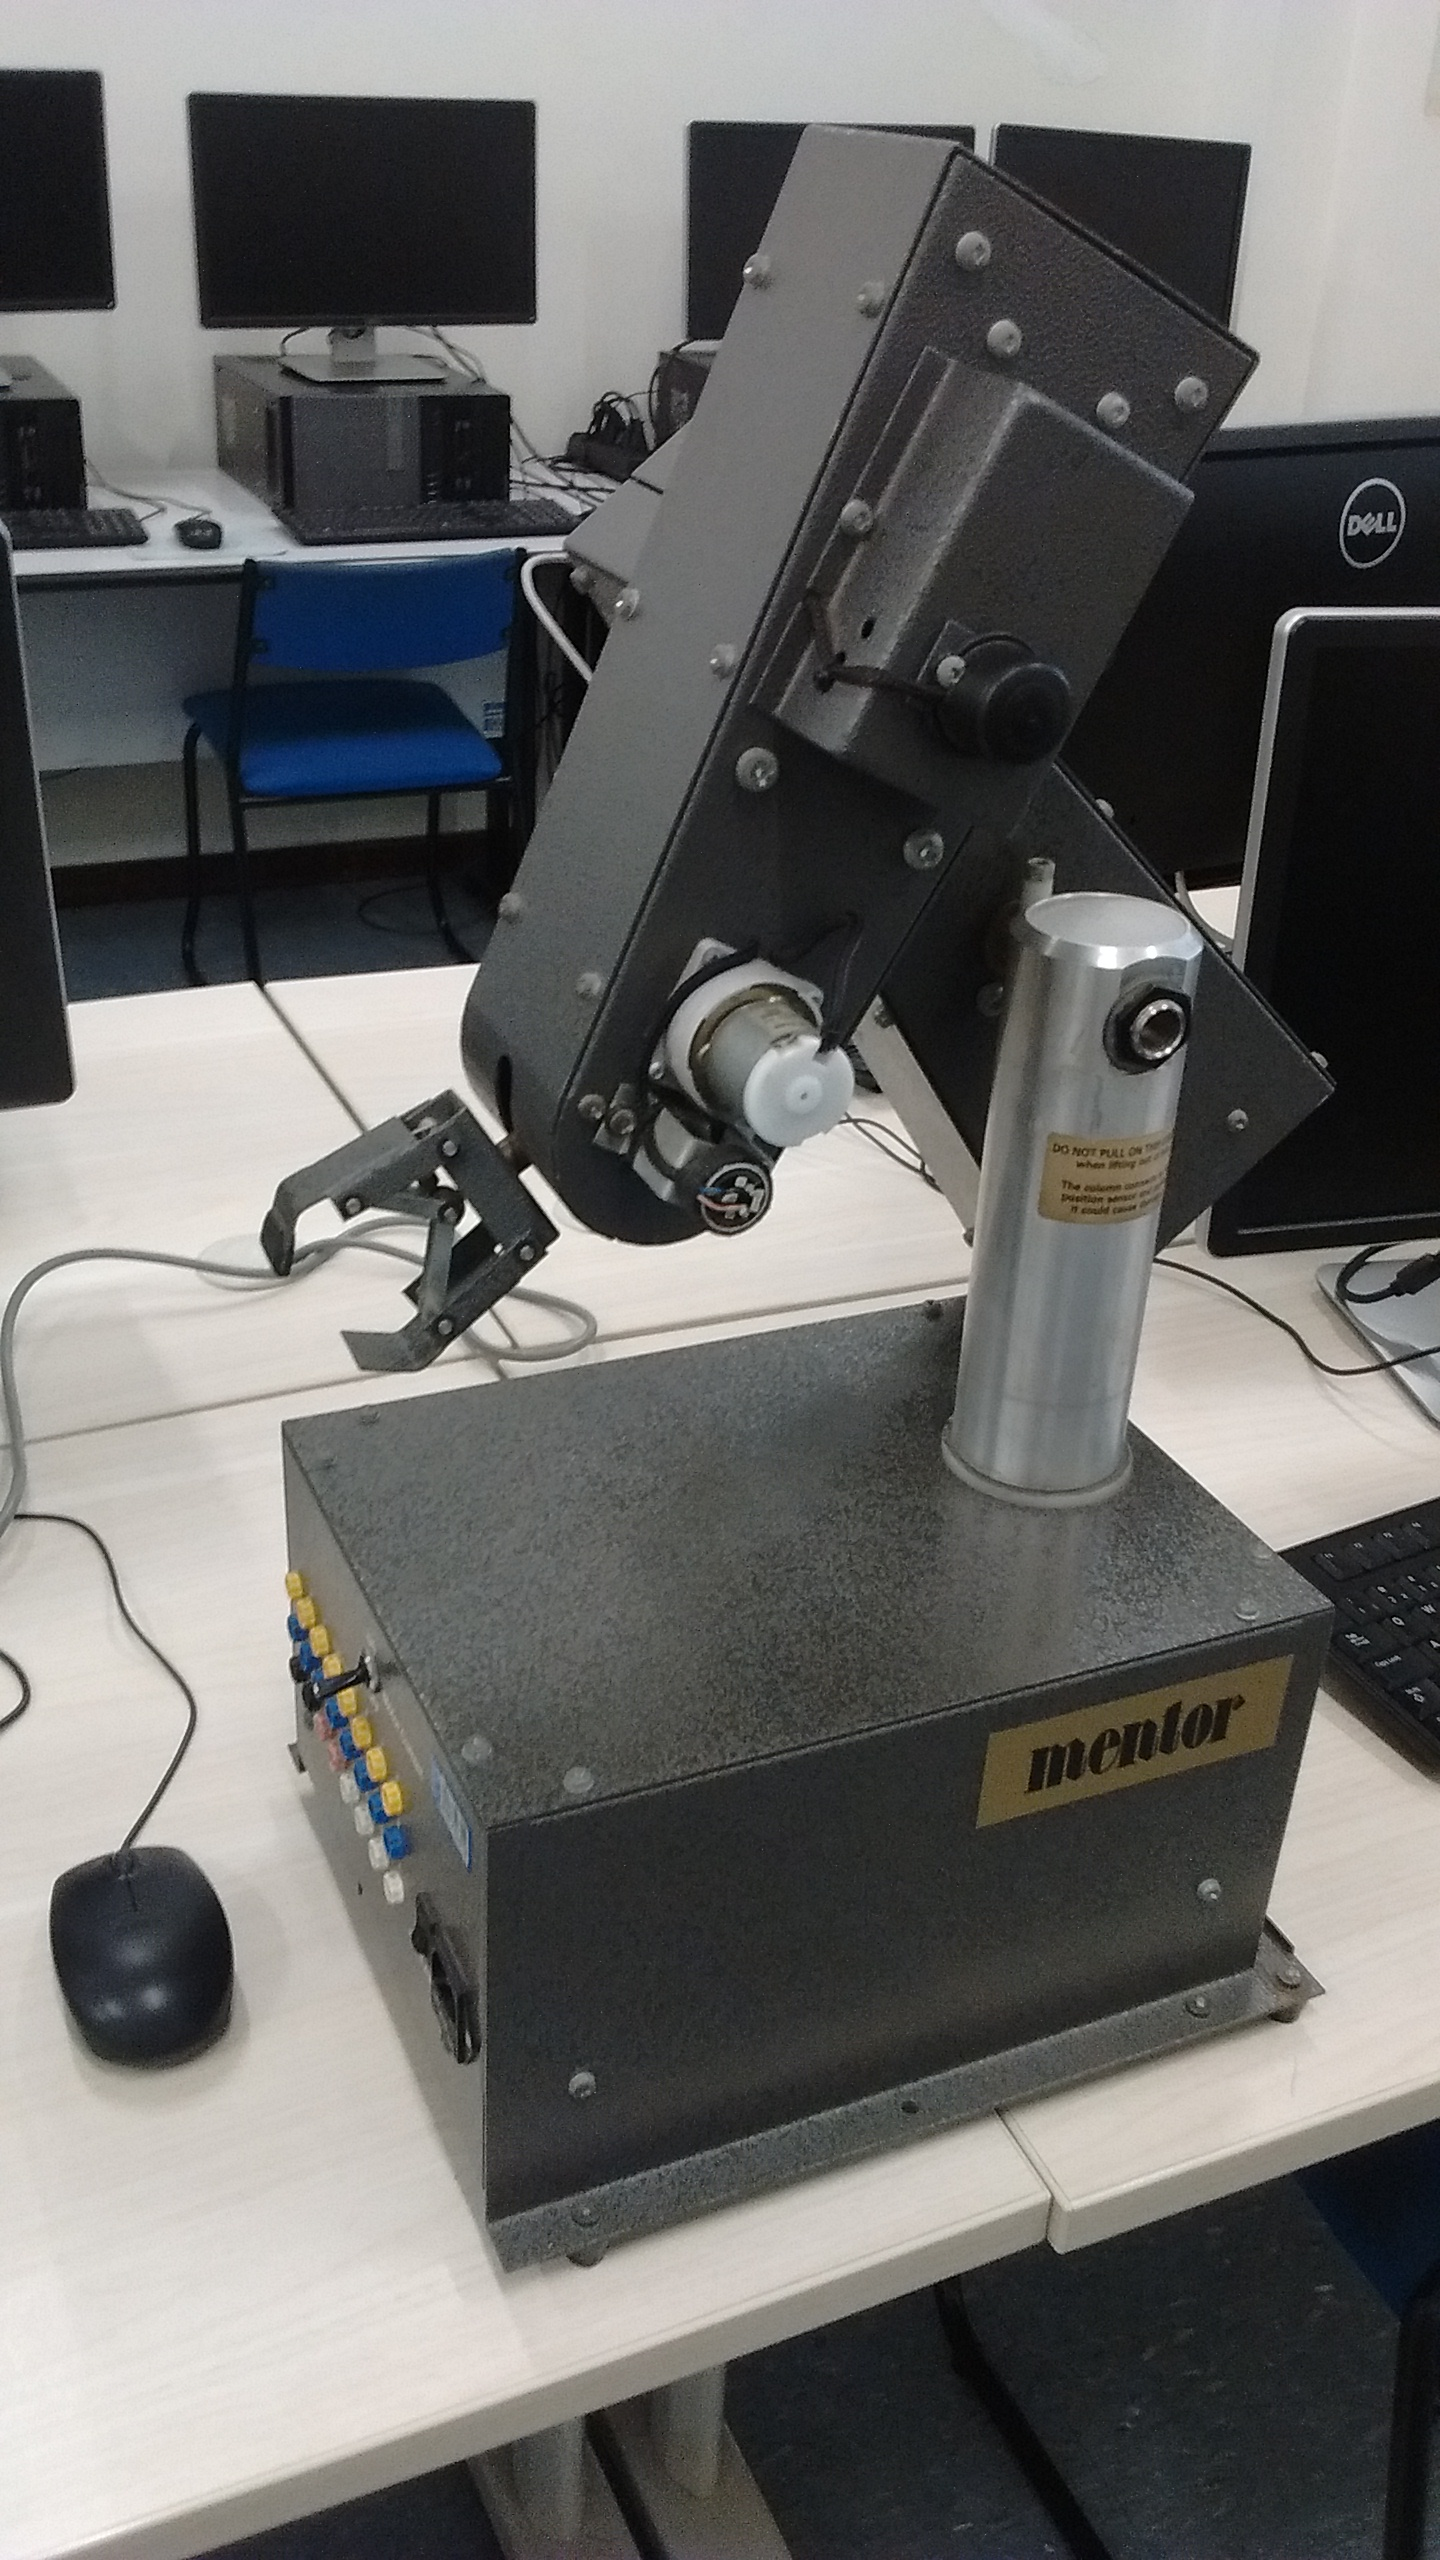
\includegraphics[keepaspectratio=true, width=0.9\linewidth]
            {img/foto-manipulador-preto.jpg}
        \fonte{http://arquivo.eng.br/robotica}
        \label{fig:fotoManipuladorMentor}
    \end{minipage}
    \begin{minipage}{.5\textwidth}
        \centering
        \caption{Manipulador robótico RD5NT}
        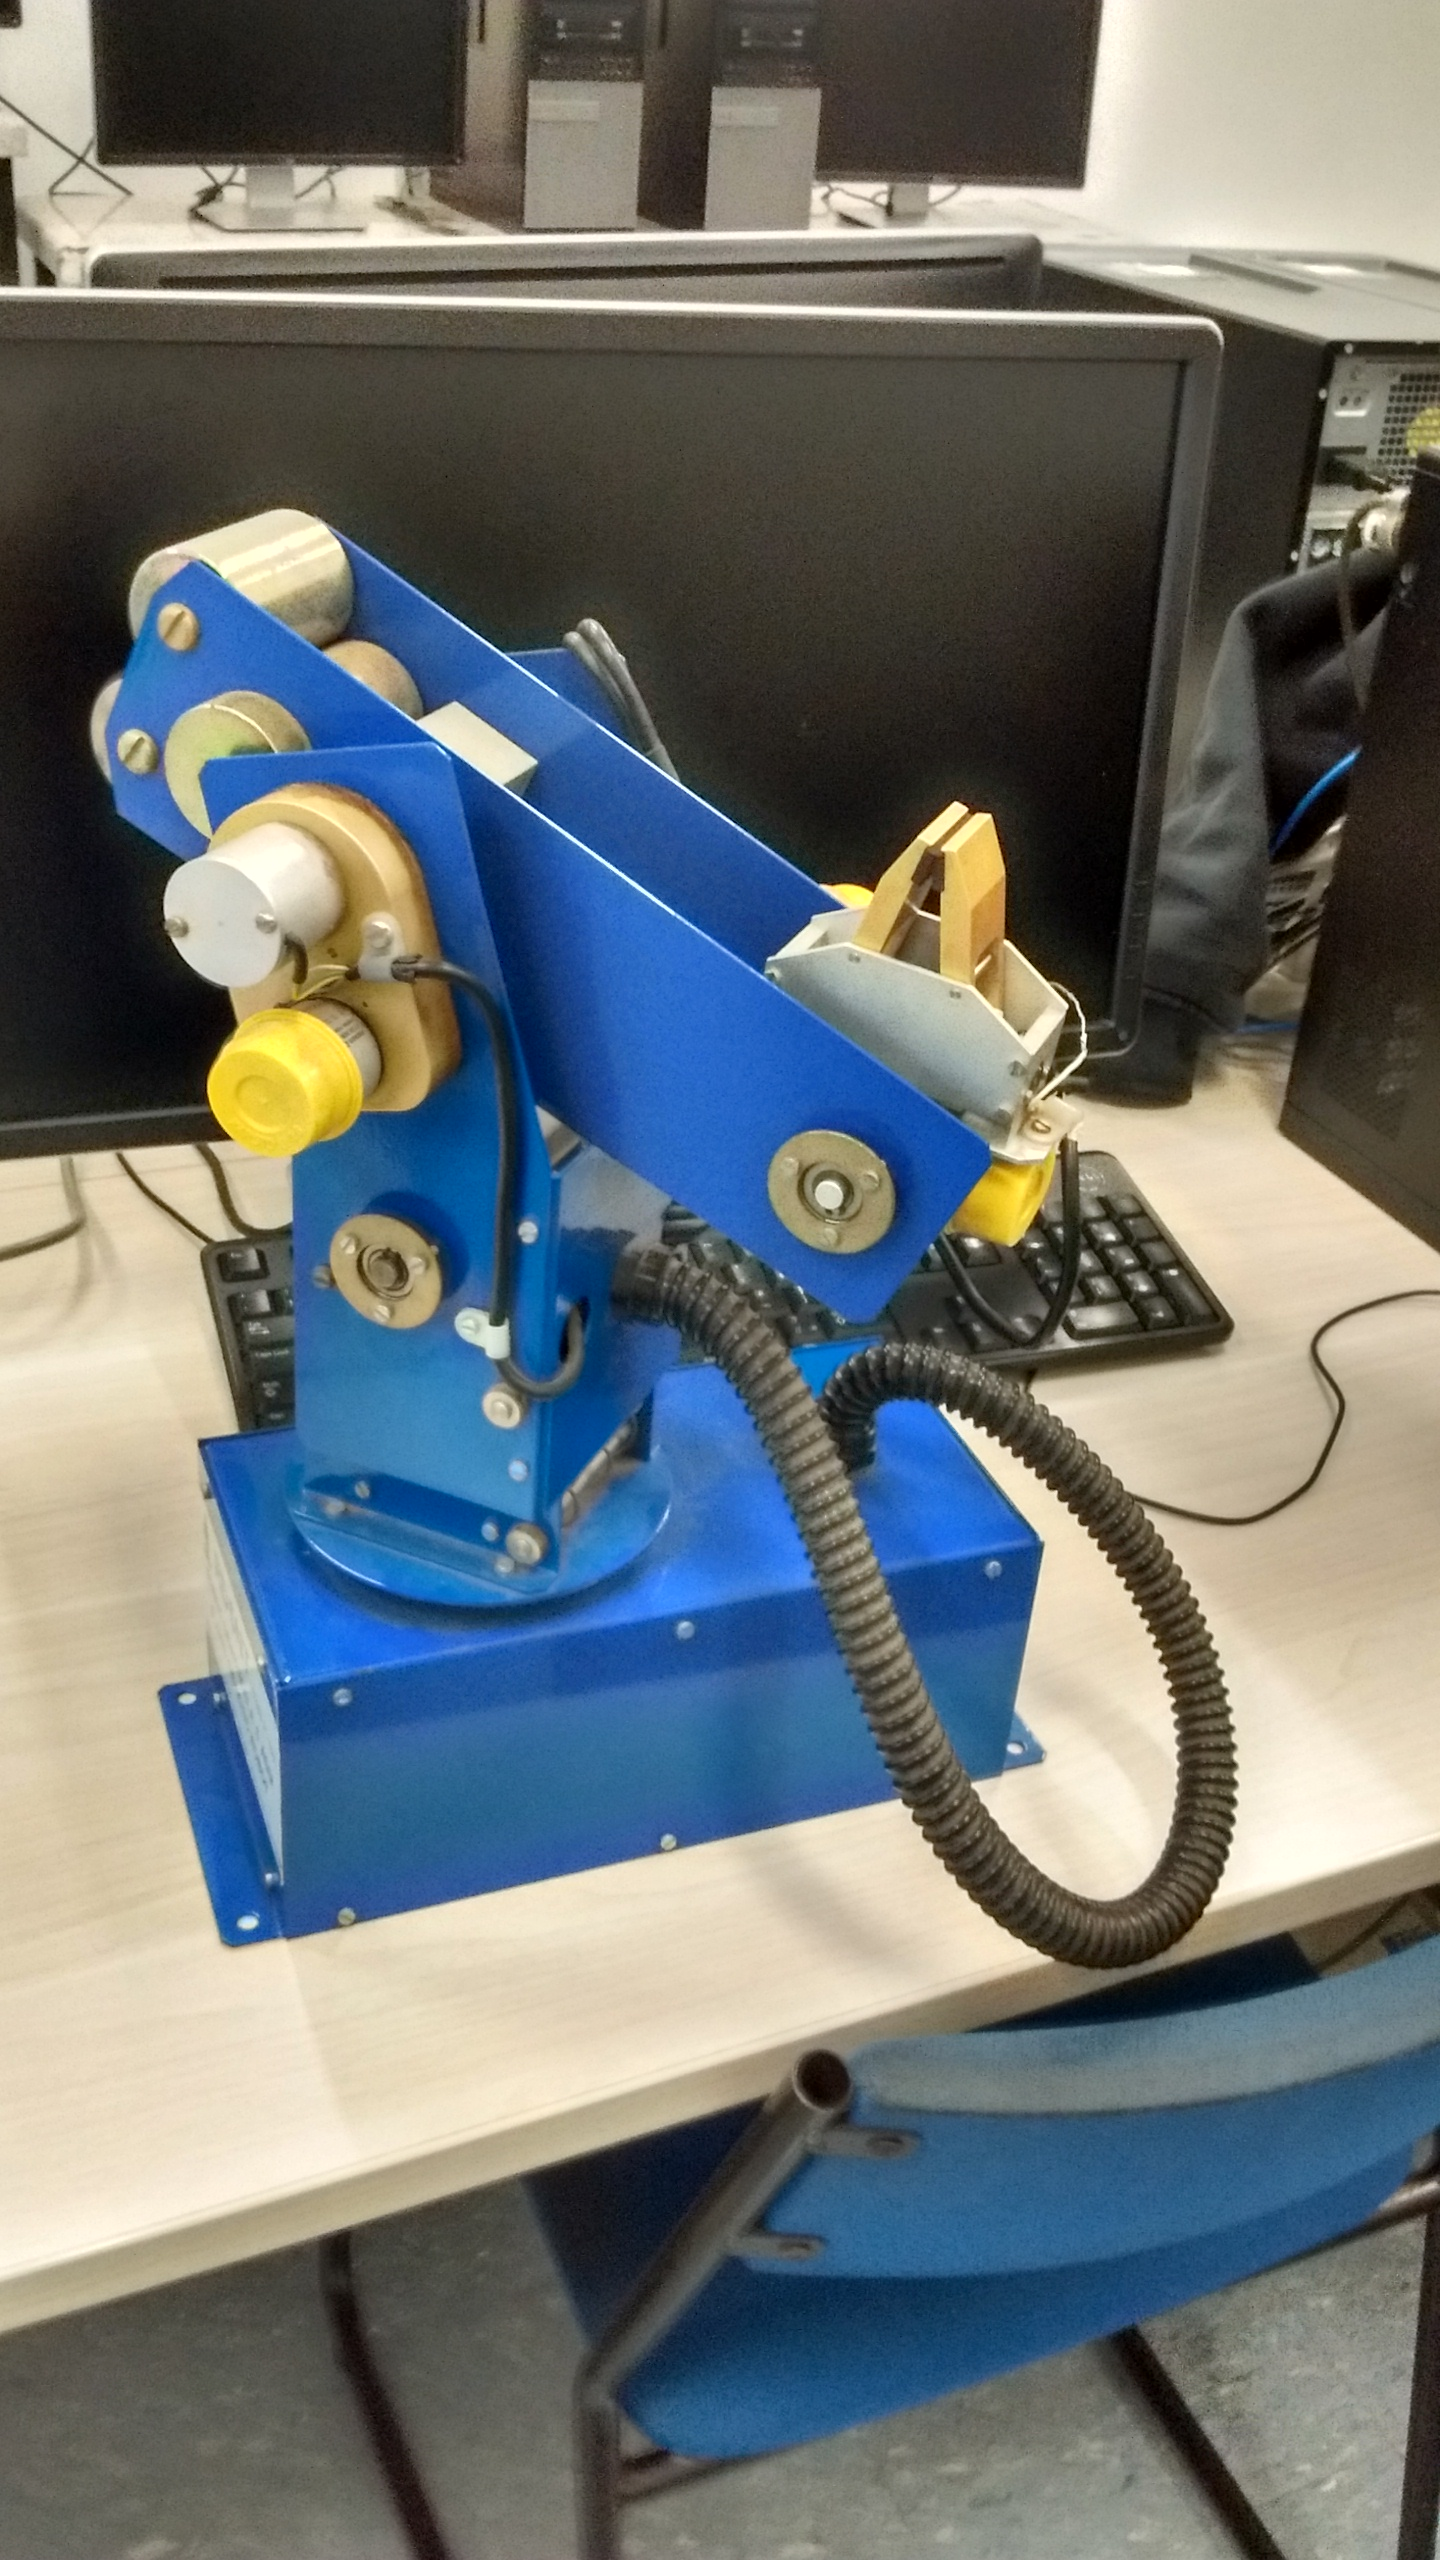
\includegraphics[keepaspectratio=true, width=0.9\linewidth]
            {img/foto-manipulador-RD5NT.jpg}
        \fonte{http://arquivo.eng.br/robotica}
        \label{fig:fotoManipuladorRD5NT}
    \end{minipage}%
\end{figure}

Foi decidido utilizar o manipulador de modelo RD5NT para o projeto, pois ele possui menos graus de liberdade na sua garra, o que facilita a implementação do algoritmo de controle.
Além disso, ele possui uma garra de tamanho adequado para pegar as peças de xadrez sem derrubar as outras peças do tabuleiro.
Apesar de não possuir caixa de redução em seus motores, isso não é um problema, pois o controle do manipulador será realizado de forma contínua.
A Figura \ref{fig:fotoBracoTabuleiro} apresenta o manipulador RD5NT ao lado de um tabuleiro de xadrez.

\begin{figure}[H]
    \centering
    \caption{Braço Robótico RD5NT ao lado de um tabuleiro de xadrez}
    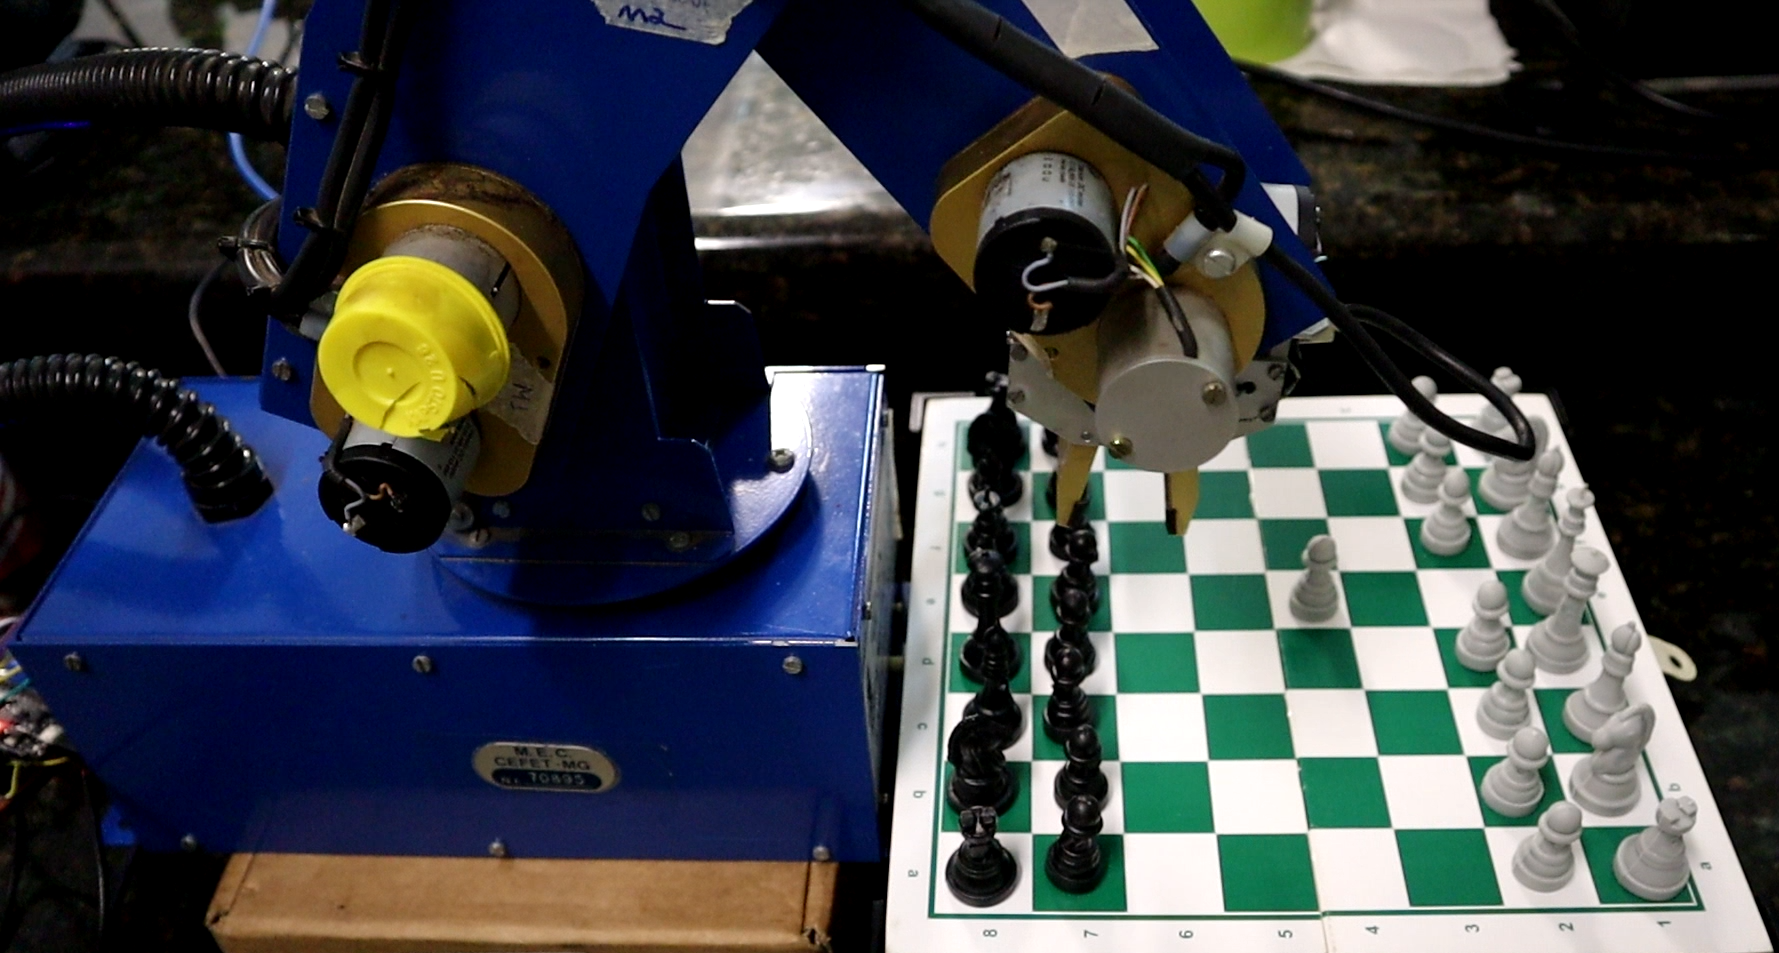
\includegraphics[keepaspectratio=true, width=0.9\textwidth]
    	{img/braco-tabuleiro.png}
    \fonte{Do próprio autor}
    \label{fig:fotoBracoTabuleiro}
\end{figure}

\subsection[Manete para o jogador]{Manete para o jogador}
\label{sub:maneteJogador}

Para que o jogador possa interagir com o manipulador, foi decidido utilizar uma manete de modelo \textit{batpad}, que possui dois \textit{joysticks}, conforme a Figura \ref{fig:fotoManeteJogador}.

Esses \textit{joysticks} devem ser alimentados com 3,3 ou 5 V e permitem a leitura de posição em duas dimensões, através de sinais analógicos.
Eles também possuem um botão que envia um sinal digital ao ser pressionado.

\begin{figure}[H]
    \centering
    \caption{Manete para o jogador}
    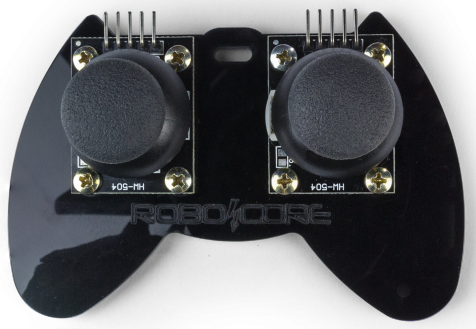
\includegraphics[keepaspectratio=true, width=0.5\textwidth]
    	{img/foto-controle-jogadores.png}
    \fonte{https://www.robocore.net/acessorios-robocore/controle-batpad}
    \label{fig:fotoManeteJogador}
\end{figure}

\subsection[Microcontrolador]{Microcontrolador}
\label{sub:microcontrolador}

Para realizar a integração entre a manete e o manipulador, foi decidido utilizar um microcontrolador ESP32, conforme a Figura \ref{fig:fotoESP32}.
Esse microcontrolador possui um \textit{clock} de 240MHz, 4MB de memória \textit{flash} e 320KB de memória \textit{RAM}.
Ele apresenta ao todo 34 pinos que podem ser utilizados como entrada ou saída, e suporta sinais analógicos e digitais \cite{esp32_datasheet}.

Para permitir o controle manual do manipulador robótico, o microcontrolador faz a leitura dos sinais analógicos e digitais provenientes da manete com alguns de seus 18 canais de \textit{ADC} (\textit{Analog to Digital Converter})[Conversor Analógico Digital].
E para permitir o controle automático, ele recebe sinais de controle de um computador através de um cabo USB.
A partir desses sinais, o ESP32 realiza o cálculo das posições desejadas de cada junta do manipulador.

Para controlar os motores, o microcontrolador primeiramente faz a leitura dos sinais analógicos provenientes dos potenciômetros de cada junta.
A partir desses sinais, é possível determinar a posição atual de cada junta.
Com base na posição atual e na posição desejada, o microcontrolador envia um sinal de controle para os motores do manipulador robótico, 
conforme apresentado na Figura \ref{fig:diagramaControle}.

\begin{figure}[H]
    \centering
    \caption{Diagrama de controle do sistema}
    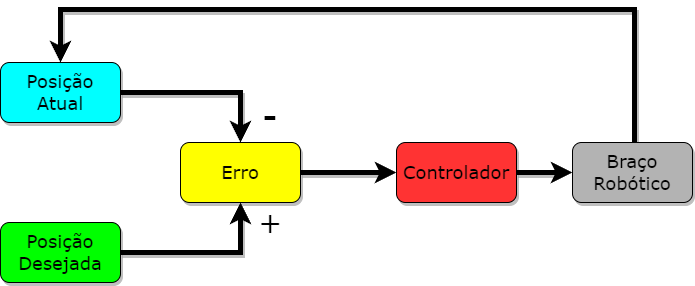
\includegraphics[keepaspectratio=true, width=0.9\textwidth]
    	{img/Diagrama Controle.png}
    \fonte{Do próprio autor}
    \label{fig:diagramaControle}
\end{figure}

Os sinais de controle são digitais do tipo \textit{PWM} (\textit{Pulse Width Modulation}), que variam de 0 a 3,3 V e possibilitam o controle da velocidade de rotação dos motores através da variação da tensão média.
Essa variação é feita através da escolha de valores diferentes de \textit{Duty Cycle} [Ciclo de Trabalho], que podem variar de 0\% a 100\%, e determinam a largura de pulso do sinal, conforme ilustrado na Figura \ref{fig:pwm}.
Valores maiores de \textit{Duty Cycle} resultam em maior velocidade de rotação do motor, pois o sinal permanece em nível alto por um período maior de tempo.
Por outro lado, valores menores de \textit{Duty Cycle} resultam em menor velocidade de rotação do motor, pois o sinal permanece em nível alto por um período menor de tempo.
Para definir o sentido de rotação do motor, foi utilizado um sinal digital que indica se ele deve girar no sentido horário ou anti-horário.

\begin{figure}[H]
    \begin{minipage}{.5\textwidth}
        \centering
        \caption{Largura do pulso do sinal de controle}
        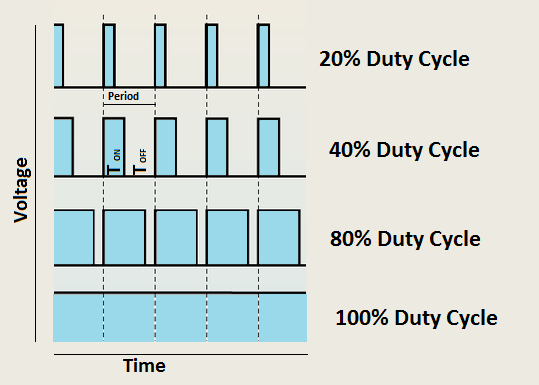
\includegraphics[keepaspectratio=true, width=0.95\textwidth]
            {img/pwm.png}
        \fonte{https://create.arduino.cc/projecthub/muhammad-aqib/arduino-pwm-tutorial-ae9d71}
        \label{fig:pwm}
    \end{minipage}
    \begin{minipage}{.5\textwidth}
        \centering
        \caption{Microcontrolador ESP32}
        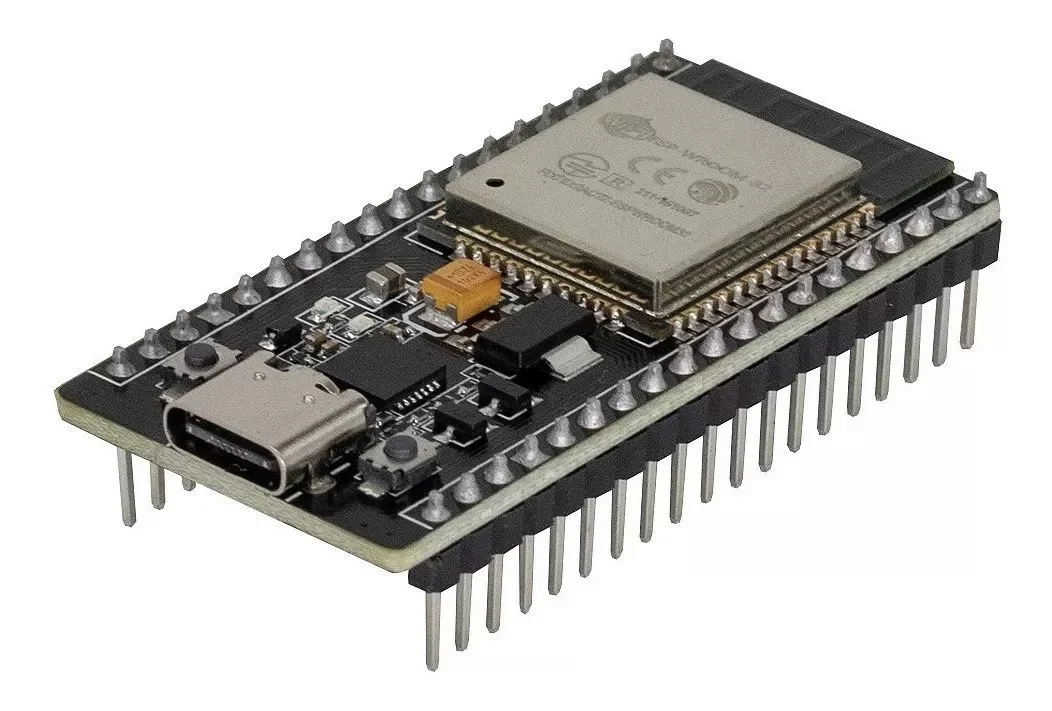
\includegraphics[keepaspectratio=true, width=0.95\textwidth]
            {img/foto-esp32.png}
        \fonte{https://www.robobuilders.com.br/nodemcu-esp32-38-pinos-devkit}
        \label{fig:fotoESP32}
    \end{minipage}%
\end{figure}

\subsection[Circuito de acionamento]{Circuito de acionamento}
\label{sub:circuitoAcionamento}

Para controlar os motores do manipulador, é necessário o uso de um circuito de acionamento para converter os sinais de baixa potência provenientes do microcontrolador em sinais de maior potência que movimentam as juntas do manipulador robótico.
Esse circuito é alimentado com 12 V, recebe sinais digitais de direção e de \textit{PWM} do ESP32 e envia sinais digitais para os motores do manipulador.

Para obter essa funcionalidade, foi decidido utilizar módulos de ponte H, que são circuitos integrados (CI) utilizados para aplicar uma tensão variável a um componente por meio de um sinal de \textit{PWM}.
Eles também permitem alterar a direção em que a corrente é aplicada no componente, o que possibilita inverter o sentido de rotação de um motor \cite{h_bridge}.
A Figura \ref{fig:ponteH} apresenta um módulo de ponte H disponível no mercado, que utiliza o CI L298N.

\begin{figure}[H]
    \centering
    \caption{Módulo de ponte H}
    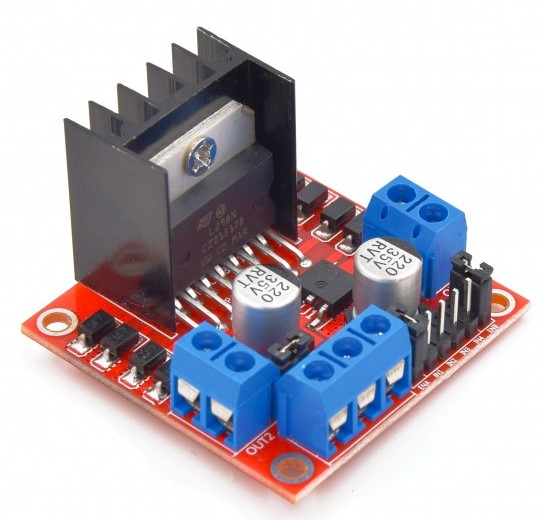
\includegraphics[keepaspectratio=true, width=0.5\textwidth]
    	{img/ponte-h.jpg}
    \fonte{https://www.smart-prototyping.com/L298N-Dual-H-bridge-Motor-Driver-Board}
    \label{fig:ponteH}
\end{figure}

\subsection[Computador]{Computador}
\label{sub:computador}

Para gerenciar o jogo de xadrez, foi decidido utilizar um computador.
Ele é responsável por implementar a lógica do jogo de xadrez e enviar sinais de controle para o ESP32, que por sua vez controla o manipulador robótico.

Para realizar a comunicação entre o computador e o ESP32, pode ser usado o protocolo serial, através de um cabo USB.
Através dele o computador envia sinais indicando para qual casa do tabuleiro o manipulador deve mover, e quando ele deve pegar ou soltar uma peça.
Por outro lado, o ESP32 envia sinais indicando quando o movimento foi finalizado e, no modo manual, qual movimento o jogador deseja realizar.

Para implementar as regras do jogo, é necessário desenvolver um \textit{software} para interagir com uma \textit{engine} de xadrez.
Essa \textit{engine} é um \textit{software} que implementa as regras do jogo e permite que o computador jogue xadrez contra um humano ou contra outro computador.
Ao integrar o \textit{software} desenvolvido com uma \textit{engine}, é possível verificar quais movimentos são válidos, determinar qual movimento será jogado pelo computador e identificar quando o jogo terminou.
Por fim, o computador também é responsável por converter um movimento em uma sequência de comandos que devem ser enviados ao ESP32.

\section[Projeto do sistema]{Projeto do sistema}
\label{sec:projetoSistema}

Após a definição de todos os equipamentos a serem utilizados, foi feito o projeto do sistema,
indicando como os componentes devem ser conectados.

A manete deve ser alimentada com 3,3 V e ser conectada ao ESP32 para permitir a leitura dos sinais de entrada.
Essa conexão é realizada com 10 cabos, sendo 5 para cada \textit{joystick} com seu respectivo botão.

O circuito de acionamento deve ser alimentado com 12 V e também deve ser conectado ao ESP32 para receber os sinais de controle.
Essa conexão é realizada com 10 cabos, 2 para o controle de cada junta do manipulador robótico.
Essa circuito também deve ser conectado aos motores do manipulador robótico, também com 10 cabos, 2 para cada junta.

O manipulador robótico deve ser conectado ao ESP32 para o envio dos sinais de posição de cada junta.
Essa conexão é realizada com 5 cabos, um para cada junta.

Por fim, o ESP32 deve ser alimentado com 3,3 V e deve ser conectado a um computador para a implementação da lógica do jogo.

A montagem do sistema é mostrada na Figura \ref{fig:montagemSistema}.

\begin{figure}[H]
    \centering
    \caption{Montagem do sistema}
    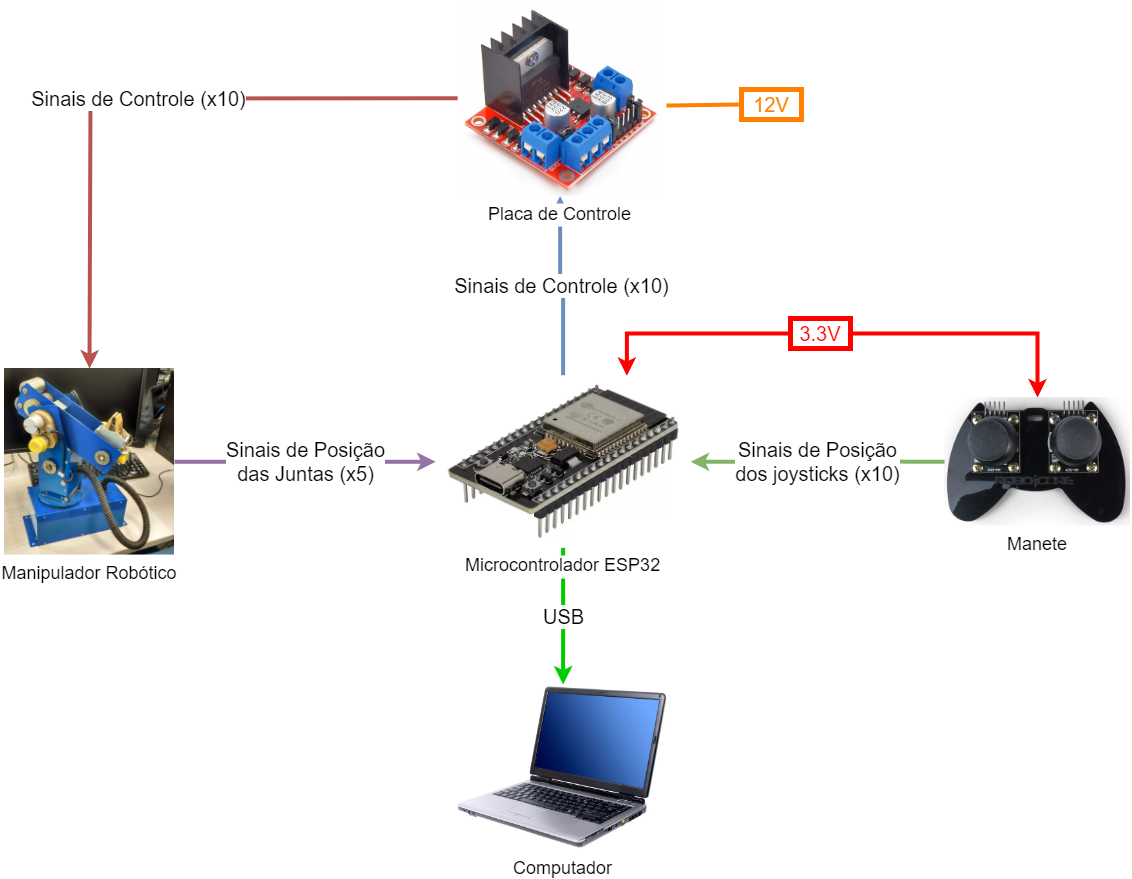
\includegraphics[keepaspectratio=true, width=0.8\textwidth]
    	{img/projeto-sistema.png}
    \fonte{Do próprio autor}
    \label{fig:montagemSistema}
\end{figure}




\chapter[Desenvolvimento]{Desenvolvimento}
\label{cap:desenvolvimento}

Após o planejamento do projeto, foi feito o desenvolvimento de cada etapa.
Inicialmente, foi feito o desenvolvimento do circuito de acionamento para poder acionar os motores.
Em seguida, o \textit{software} para o microcontrolador foi desenvolvido para realizar a leitura dos dados da manete e controlar o manipulador robótico.
Em sequência, foi desenvolvido o \textit{software} para o computador, que implementa a lógica do jogo de xadrez.
Por fim, foi feita uma análise do desempenho do sistema.

\section[Desenvolvimento do circuito de acionamento]{Desenvolvimento do circuito de acionamento}
\label{sec:desenvolvimentoCircuitoAcionamento}

Primeiramente, foi feito o desenvolvimento do circuito de acionamento dos manipuladores, pois ele é necessário para as próximas etapas do projeto.
Para isso, foi necessário definir quais componentes utilizar e como conectá-los.

Conforme descrito na subseção \ref{sub:circuitoAcionamento}, o circuito de acionamento deve utilizar uma ponte H para o controle de cada junta.
Para isso, foi escolhido o CI L293D, que possui duas pontes H e suporta tensões de 12V.
Como é necessário controlar 6 motores, foram utilizados 3 CI L293D.

Para simplificar o controle e evitar problemas de acionamento duplo das entradas das pontes H, foi utilizado o CI 74LS02 como um inversor lógico.
Dessa forma, o circuito de acionamento possui para cada junta uma entrada de \textit{Enable} para ligar/desligar o acionamento da junta, e uma porta de \textit{Direction} para definir a direção de movimentação dela.
A partir dessas entradas, o CI L293D é acionado e o motor é controlado.
A Figura \ref{fig:esquematicoSimplificado} mostra o esquemático simplificado de um CI L293D e um CI 74LS02.

\begin{figure}[H]
    \centering
    \caption{Esquemático simplificado de um CI L293D e um CI 74LS02}
    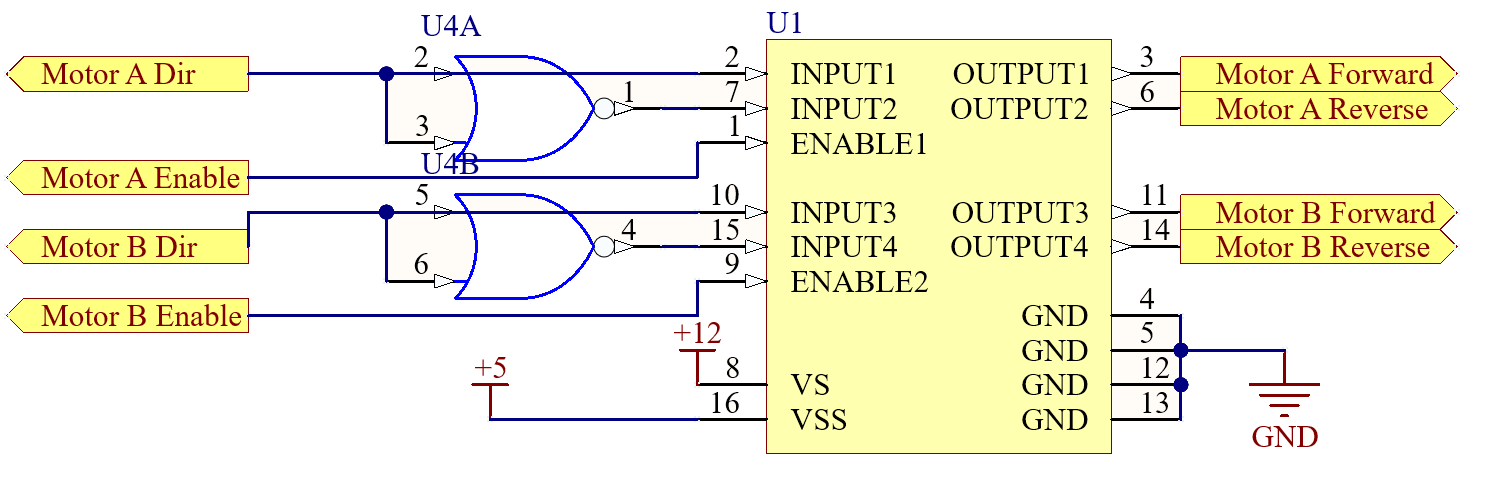
\includegraphics[keepaspectratio=true, width=0.9\textwidth]
    	{img/placa-controle-esquematico-simplificado.png}
    \fonte{Do próprio autor}
    \label{fig:esquematicoSimplificado}
\end{figure}

Com os componentes principais definidos foi feito o desenvolvimento do esquemático do circuito de acionamento com o auxílio do \textit{software} \textit{Altium Designer}.
O Apêndice \ref{apendice:esquematicoCircuitoAcionamento} mostra o esquemático completo do circuito de acionamento.
Nesse esquemático foram adicionados resistores de \textit{pulldown} para garantir que as entradas dos CI L293D e 74LS02 permaneçam em nível lógico baixo caso não estejam conectadas ao microcontrolador.
Também foram adicionadas \textit{LEDs} para indicar a alimentação de 5V e 12V do circuito.

Após o desenvolvimento do esquemático, foi feita a montagem da Placa de Circuito Impresso (PCB), ainda com o auxílio do \textit{software} \textit{Altium Designer}.
Para isso, os componentes foram posicionados no \textit{layout} da placa, tendo em vista a economia de espaço e a necessidade de manter os componentes próximos para facilitar sua conexão.
Em seguida, as trilhas e vias que realizam a conexão dos componentes foram desenhadas. 
Para permitir a conexão de todos os componentes, foi necessário utilizar uma placa com 2 camadas.
A Figura \ref{fig:circuitoAcionamentoLayout} mostra o \textit{layout} final do circuito de acionamento.

Com o \textit{layout} finalizado, foi feita a produção da PCB de forma manual.
Para isso, o negativo do \textit{layout} foi impresso em uma folha de transparência.
Depois, uma placa de circuito impresso de duas camadas foi cortada no tamanho desejado.

Em seguida, foi feita a transferência do \textit{layout} para a placa.
Para isso, uma fina camada de tinta fotossensível destinada para PCB foi aplicada sobre a placa.
Essa tinta foi pré-curada a 75$^{\circ}$C durante 15 minutos com o auxílio de uma base de aquecimento, para garantir que ela não se descolasse da placa.
Após a pré-cura, a tinta foi exposta à luz ultravioleta por 3 minutos, utilizando a transparência com o \textit{layout} como máscara.
Em seguida, a placa foi submersa em uma solução de carbonato de sódio para realizar a revelação do \textit{layout}.
Após a placa ser revelada, a tinta foi curada a 85$^{\circ}$C durante 30 minutos.

Esse processo de transferência do \textit{layout} foi repetido para a segunda camada da placa.
Em seguida, foi utilizada uma solução de percloreto de ferro para corroer as áreas de cobre que não receberam tinta.
Após a corrosão, a placa foi mergulhada em uma solução de hidróxido de sódio para remover a tinta.

Após a corrosão da PCB, foi feita a perfuração das vias e dos furos para os componentes.
Por fim, foi feita a soldagem dos componentes na placa e a conexão das vias.
A Figura \ref{fig:circuitoAcionamento} mostra o circuito de acionamento montado.

\begin{figure}[H]
    \begin{minipage}{.45\textwidth}
        \centering
        \caption{Layout do circuito de acionamento}
        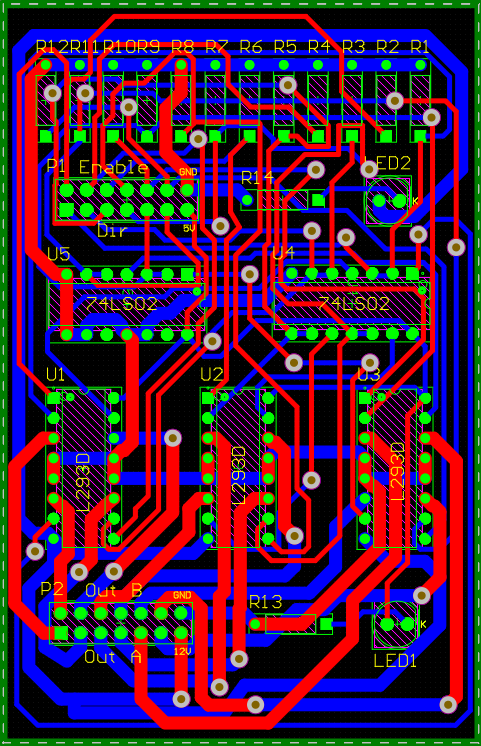
\includegraphics[keepaspectratio=true, width=0.9\linewidth]
            {img/placa-controle-layout.png}
        \fonte{Do próprio autor}
        \label{fig:circuitoAcionamentoLayout}
    \end{minipage}
    \begin{minipage}{.10\textwidth}
    \end{minipage}
    \begin{minipage}{.45\textwidth}
        \centering
        \caption{Circuito de acionamento produzido}
        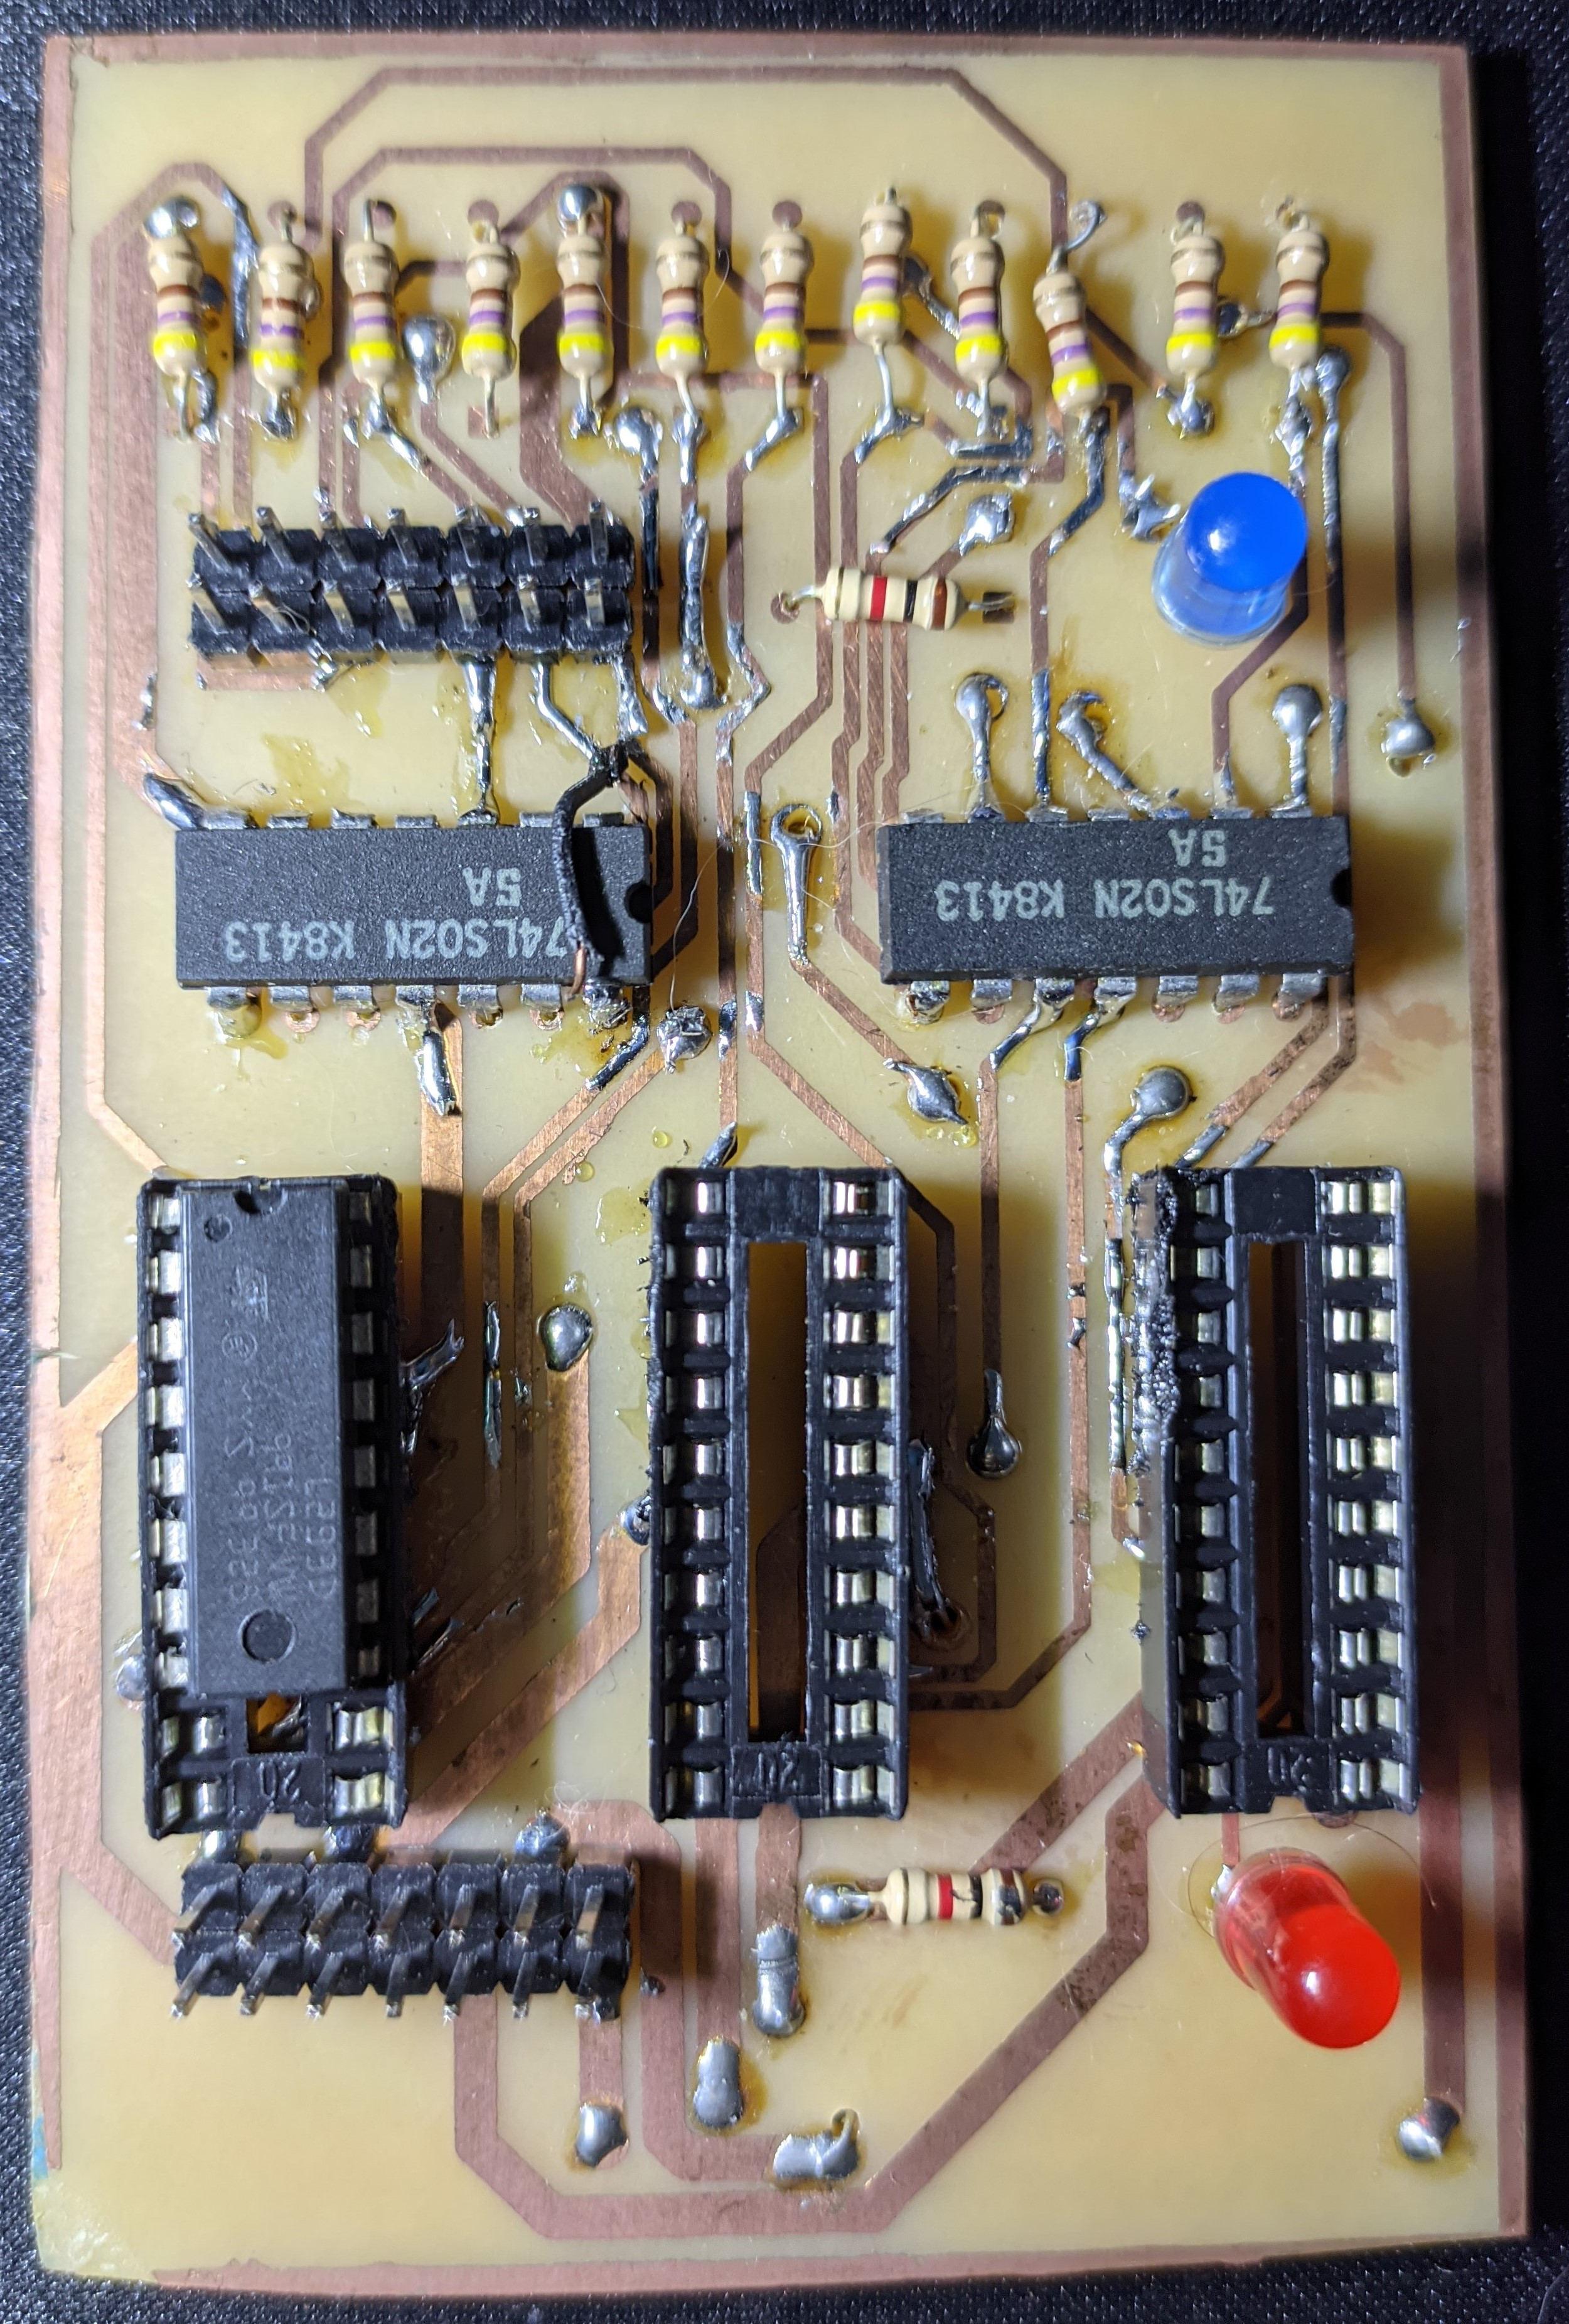
\includegraphics[keepaspectratio=true, width=0.95\linewidth]
            {img/placa-controle.jpg}
        \fonte{Do próprio autor}
        \label{fig:circuitoAcionamento}
    \end{minipage}
\end{figure}

\section[Leitura de comandos da manete]{Leitura de comandos da manete}
\label{sec:leituraComandosManete}

Após a montagem da placa de controle, foi iniciado o desenvolvimento do \textit{software} para o microcontrolador,
utilizando o \textit{software} \textit{PlatformIO}.

Inicialmente, foi implementada uma funcionalidade para realizar a leitura dos dados da manete que, 
conforme descrito na subseção \ref{sub:maneteJogador}, possui dois \textit{joysticks} com dois eixos e um botão cada.

Para realizar a leitura dos eixos dos \textit{joysticks}, foram utilizadas as entradas analógicas do microcontrolador.
Como o ESP32 utiliza um conversor analógico-digital (ADC) de 12 bits, os valores lidos variam de 0 a 4095.
Valores próximos de 2048 representam a posição central do \textit{joystick}, enquanto valores próximos de 0 ou 4095 representam as posições extremas.
Para aprimorar a usabilidade da manete, foi implementada uma área de \textit{deadzone}, na qual o valor lido é considerado como zero,
para evitar que o manipulador se movimente sem a intenção do usuário.

Para realizar a leitura do botão, foi utilizada uma entrada digital.
Esses botões possuem um \textit{pull-up} interno, o que significa que o valor lido é 1 quando o botão não está pressionado e 0 quando o botão está pressionado.

Os valores lidos são armazenados em uma variável, que é utilizada por outras funcionalidades do \textit{software}.

\section[Leitura da posição das juntas]{Leitura da posição das juntas}
\label{sec:leituraPosicaoJuntas}

Para ler a posição das juntas do manipulador robótico, foi utilizado como base o \textit{software} desenvolvido anteriormente para ler os dados das manetes.

Primeiramente, foi utilizado um programa simples para medir os valores de tensão do potenciômetro de cada junta em diferentes ângulos, utilizando o módulo de \textit{ADC} do microcontrolador.
A partir disso, foi observado que a tensão de saída altera de forma aproximadamente linear com o ângulo,
e foi criada uma equação linear para cada junta, que relaciona a leitura realizada pelo microcontrolador com seu ângulo atual,
conforme os dados apresentados na Figura \ref{fig:leituraJuntas}.

\begin{figure}[H]
    \centering
    \caption{Leitura da posição das juntas}
    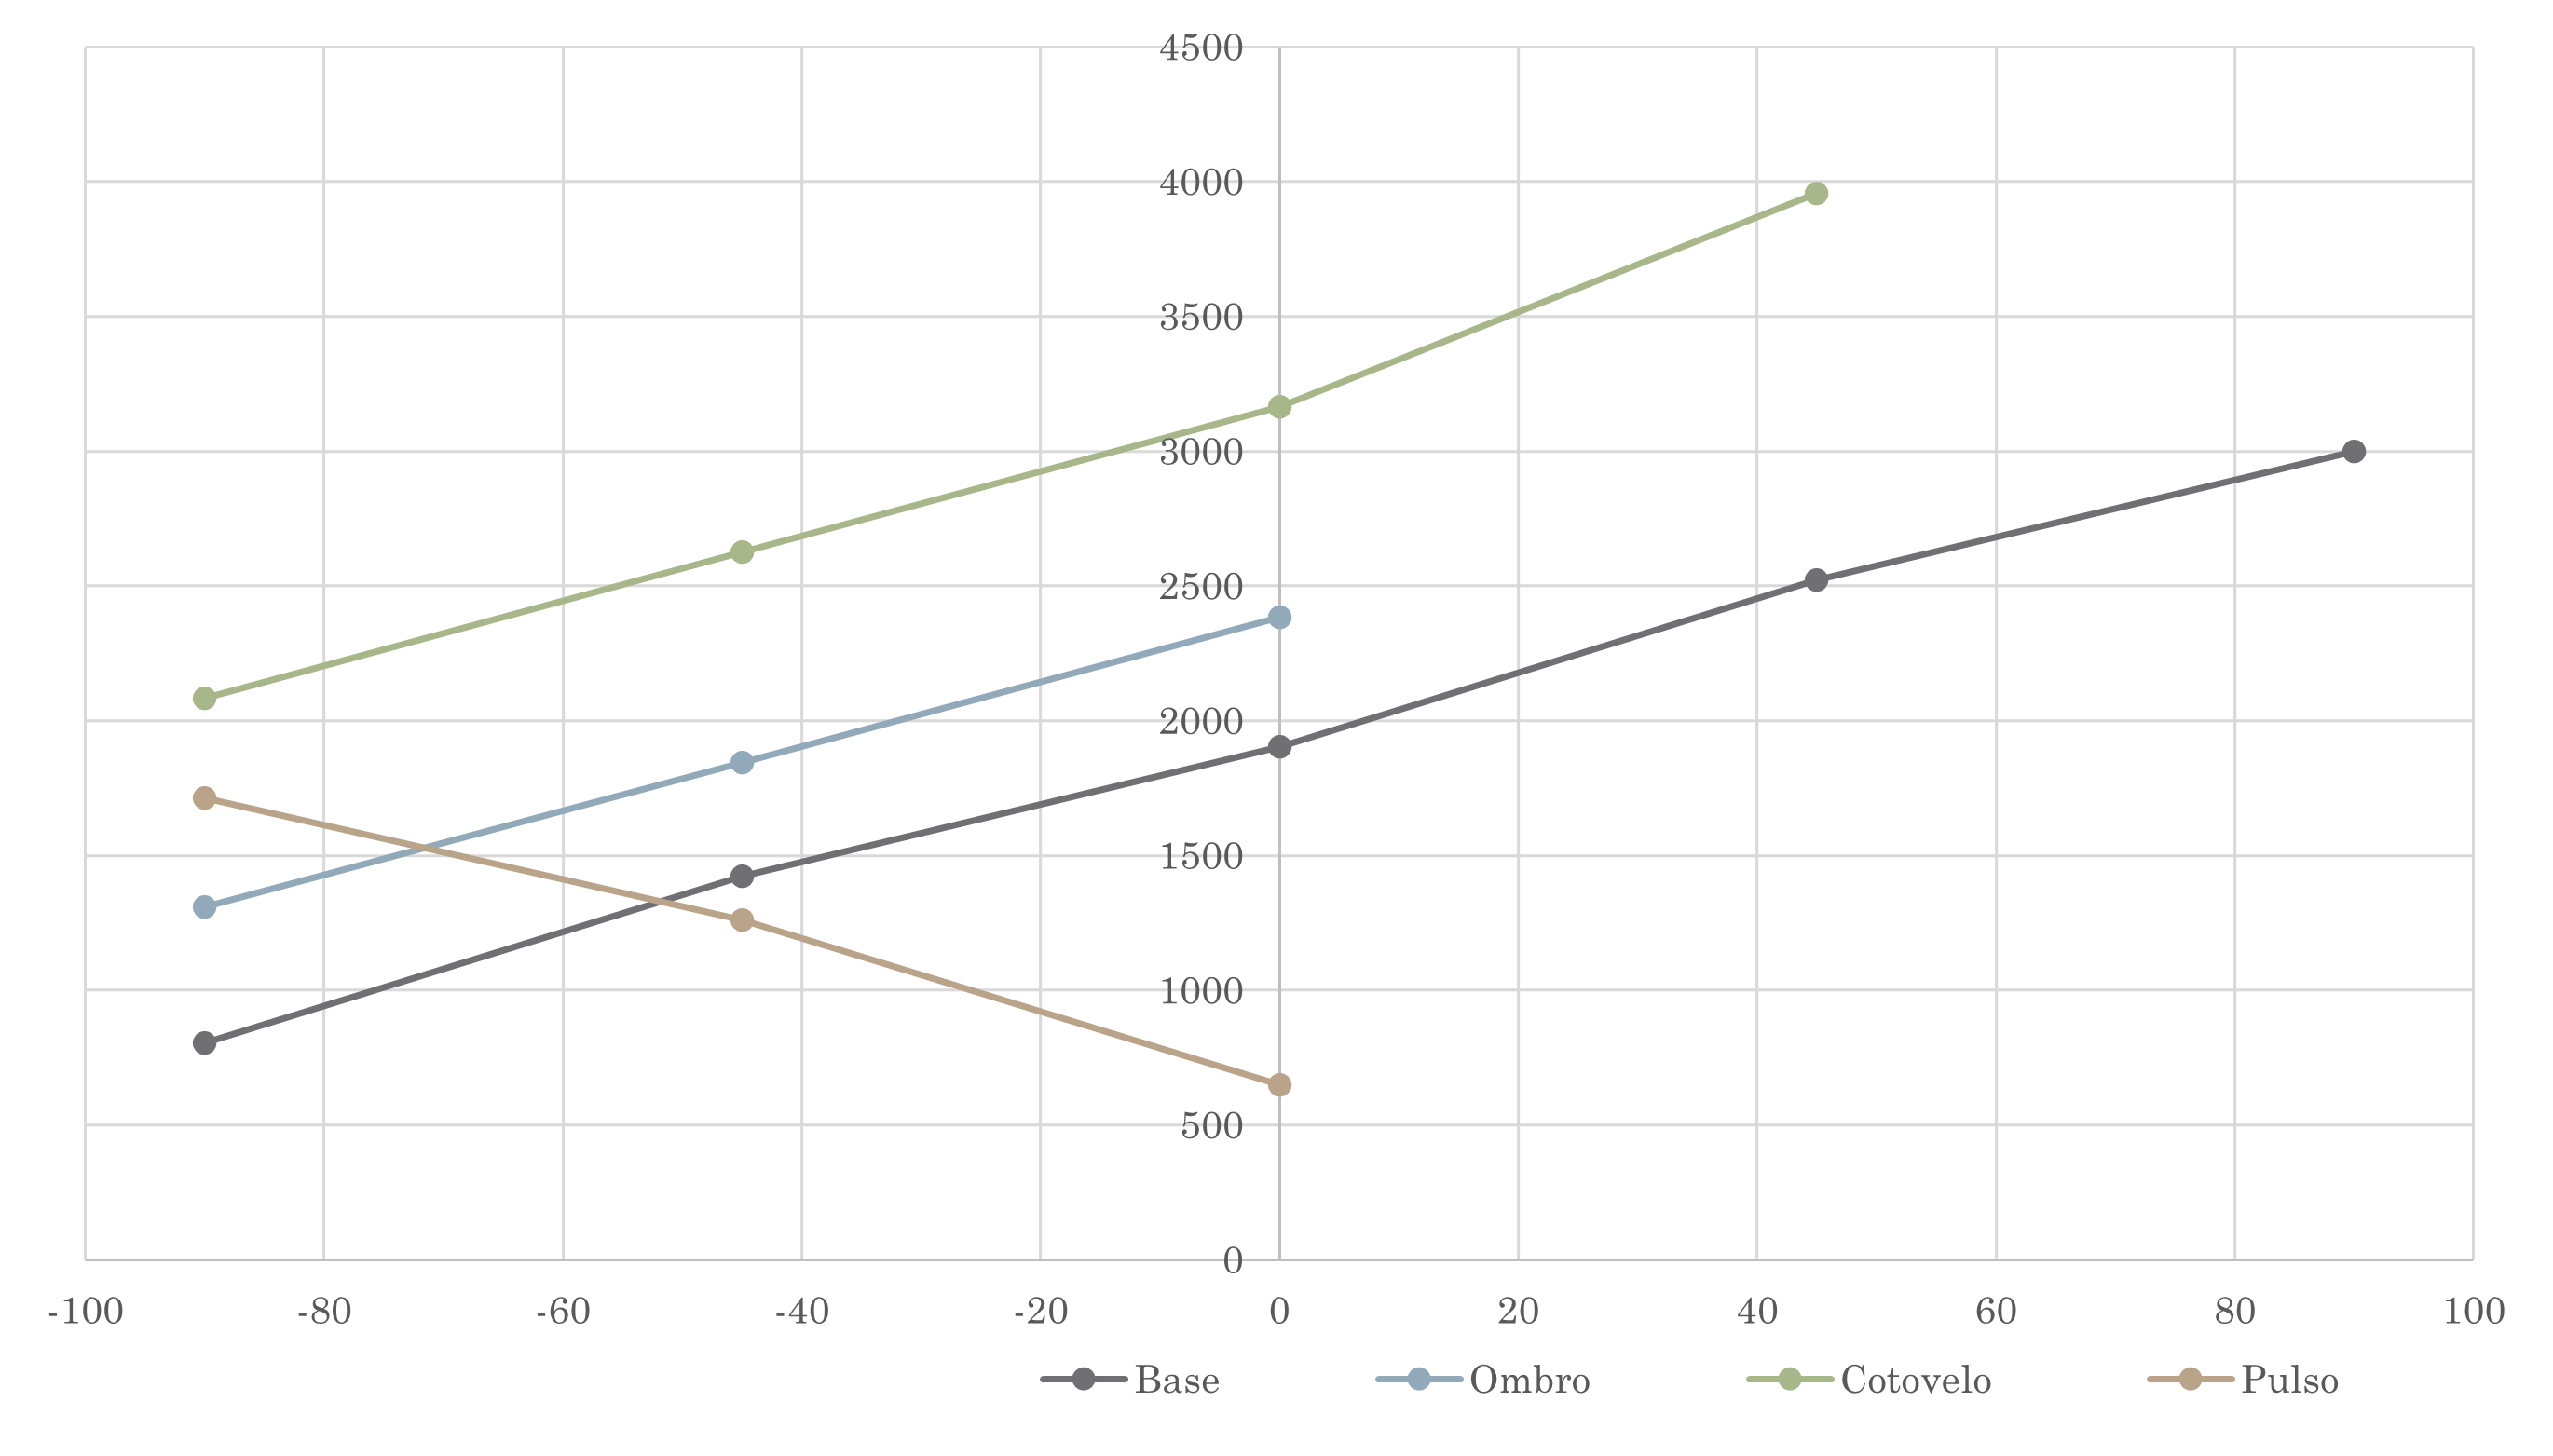
\includegraphics[keepaspectratio=true, width=\textwidth]
    	{img/leitura-juntas.png}
    \fonte{Do próprio autor}
    \label{fig:leituraJuntas}
\end{figure}

Com base nessas equações, foi implementada uma funcionalidade para calcular os valores que devem ser lidos pelo ESP32 quando o manipulador robótico estiver em uma determinada configuração.

\section[Controle dos motores]{Controle dos motores}
\label{sec:controleMotores}

O controle dos motores, responsável por mover o manipulador robótico para que ele atinja uma determinada configuração,
foi incorporado no \textit{software} desenvolvido na seção anterior.

Para isso, foi implementado um controlador digital PID no microcontrolador ESP32.
Esse algoritmo realiza a leitura dos valores de tensão de cada junta e obtém o erro a partir da diferença entre o valor desejado e o valor atual.
A partir desse erro, é calculada a integral dos erros até o momento e a derivada entre o erro atual e o último erro.
Por fim, esses valores (erro atual, integral dos erros e derivada do erro) são multiplicados, respectivamente, por três parâmetros (\textit{Kp}, \textit{Ki} e \textit{Kd}) e os resultados são somados.

Esse valor final é utilizado para definir os sinais de saída do microcontrolador para a placa de controle.
O módulo desse valor de saída do PID define o \textit{Duty Cycle} do sinal de \textit{PWM}, enquanto o seu sinal (positivo ou negativo) define a direção de movimentação do motor.

Depois da implementação do controlador PID foram feitos diversos testes para encontrar valores adequados para os parâmetros \textit{Kp}, \textit{Ki} e \textit{Kd}.
Para isso, foi enviado um comando para movimentar uma junta para um determinado ângulo.
Após a junta estabilizar na posição desejada, foi enviado um outro comando para movimentá-la para um ângulo diferente, distante do primeiro.
Para alguns valores dos parâmetros, foi observado um comportamento muito lento do sistema,
enquanto para outros valores foi observado um comportamento muito instável, com \textit{overshoot} e oscilações.
Depois de diversos testes, foram encontrados os valores apresentados na Tabela \ref{tab:parametrosPID},
que possibilitam um movimento relativamente rápido e estável do manipulador robótico.
Durante esses testes, foi observado um comportamento instável do sistema para valores altos de \textit{Kd},
portanto foi necessário utilizar um valor baixo para esse parâmetro.

\begin{table}[H]
    \centering
    \caption{Parâmetros do controlador PID}
    \begin{tabular}{|c|c|c|c|}
        \hline
        \textbf{Junta} & \textbf{\textit{Kp}} & \textbf{\textit{Ki}} & \textbf{\textit{Kd}} \\
        \hline
        Torso    & 400 & 10 & 5 \\
        \hline
        Ombro    & 500 & 40 & 0 \\
        \hline
        Cotovelo & 500 & 30 & 0 \\
        \hline
        Pulso    & 100 & 2 & 0,1 \\
        \hline        
    \end{tabular}
    \fonte{Do próprio autor}
    \label{tab:parametrosPID}
\end{table}

\section[Cálculo dos ângulos desejados]{Cálculo dos ângulos desejados}
\label{sec:calculoAngulosDesejados}

Após implementar o controle do manipulador a partir dos ângulos desejados para cada junta, foi necessário desenvolver o código que realiza o cálculo da configuração necessária para que o manipulador robótico alcance uma determinada posição no espaço,
por meio da cinemática reversa.

Primeiramente, foi feita uma análise de como cada junta do manipulador robótico se movimenta.
Como pode ser observado na Figura \ref{fig:juntasManipulador},
o torso se movimenta horizontalmente, perpendicularmente ao eixo Z.
Por outro lado, o ombro, cotovelo e pulso se movimentam verticalmente, paralelamente à base do manipulador.

\begin{figure}[H]
    \centering
    \caption{Movimento das juntas do manipulador}
    \includegraphics[keepaspectratio=true, width=1\textwidth]
    	{img/juntas-manipulador.png}
    \fonte{Do próprio autor}
    \label{fig:juntasManipulador}
\end{figure}

Em seguida, foi feita uma equação para o ângulo da primeira articulação (torso).
Como essa é a única junta capaz de rotacionar perpendicularmente ao eixo Z, seu ângulo pode ser calculado de forma independente das outras juntas, 
a partir apenas dos valores de \textit{x} e \textit{y} da posição desejada, ignorando o valor de \textit{z}.
Como é possível observar na Figura \ref{fig:calculoAnguloTorso}, o ângulo dessa junta deve formar um triângulo retângulo com catetos de comprimento \textit{x} e \textit{y}.
A partir disso, o ângulo do torso ($\alpha$) pode ser calculado como:

\begin{dmath}
\label{eq:anguloTorso}
    \alpha = \arctan\left(\frac{x}{y}\right)
\end{dmath}

\begin{figure}[H]
    \centering
    \caption{Cálculo do ângulo do torso}
    \includegraphics[keepaspectratio=true, width=0.4\textwidth]
    	{img/Ângulo base.png}
    \fonte{Do próprio autor}
    \label{fig:calculoAnguloTorso}
\end{figure}

Em seguida, foi feito o cálculo dos ângulos restantes (ombro, cotovelo e pulso).
Para que seja possível pegar as peças sem interferir nas outras em casas próximas, é indispensável que a garra do manipulador esteja sempre perpendicular com o tabuleiro.
Dessa forma, apenas é necessário calcular os ângulos do ombro e do cotovelo de forma que o ombro termine nas posições \textit{x} e \textit{y} desejadas,
entretanto sua altura final deve ser igual ao \textit{z} desejado acrescentado do comprimento da garra, para que a ponta da garra esteja no \textit{z} desejado.

Com base nisso, podemos simplificar os dados necessários para calcular os ângulos do ombro ($\beta$) e do cotovelo ($\theta$).
Essa parte do manipulador deve ter um comprimento total definido pela hipotenusa do triângulo retângulo apresentado na Figura \ref{fig:calculoAnguloTorso}, com catetos x e y.
E sua altura total deve ser igual ao z desejado, subtraído dos comprimentos da garra e do torso do manipulador.
Isso pode ser visualizado mais claramente na Figura \ref{fig:visualizacaoAnguloOmbroCotovelo}.

\begin{figure}[H]
    \centering
    \caption{Visualização do ângulo do ombro e do cotovelo}
    \includegraphics[keepaspectratio=true, width=0.9\textwidth]
    	{img/visualizacao-ombro-cotovelo.png}
    \fonte{Do próprio autor}
    \label{fig:visualizacaoAnguloOmbroCotovelo}
\end{figure}

Portanto, temos as seguintes equações, que relacionam os valores de \textit{x}, \textit{y}, \textit{z}, comprimento do torso ($\overline{torso}$) e comprimento da garra ($\overline{garra}$) com o comprimento e altura do conjunto ombro-cotovelo:

\begin{dmath}
\label{eq:comprimentoOmbroCotovelo}
    comprimento = \sqrt{x^2 + y^2}
\end{dmath}

\begin{dmath}
\label{eq:alturaOmbroCotovelo}
    altura = z - \overline{torso} - \overline{garra}
\end{dmath}

A partir desses valores de comprimento e altura, o cálculo desses ângulos se reduz a um problema de cinemática inversa de um manipulador com dois graus de liberdade.
Existem duas soluções para esse tipo de problema, uma com o ângulo do segundo eixo positivo em relação ao primeiro, e outra com esse ângulo negativo.
Devido às limitações da movimentação do ombro do manipulador utilizado, foi escolhida a solução na qual o ângulo do cotovelo é negativo \cite{inverse_kinematics}.
As equações a seguir podem ser utilizadas para calcular o ângulo do ombro ($\beta$) e do cotovelo ($\theta$) a partir do comprimento e altura do conjunto ombro-cotovelo, calculados anteriormente,
assim como do comprimento do braço ($\overline{braço}$) e do antebraço ($\overline{antebraço}$).

\begin{dmath}
\label{eq:anguloCotovelo}
    \theta = -\arccos\left(\frac{comprimento^2 + altura^2 - \overline{braço}^2 - \overline{antebraço}^2}{2 \cdot \overline{braço} \cdot \overline{antebraço}}\right)
\end{dmath}

\begin{dmath}
\label{eq:anguloCotovelo}
    \beta = \arctan{\frac{altura}{comprimento}} + \arcsin\left(\frac{\overline{antebraço} \cdot \sin\left(\theta\right)}{\overline{braço} + \overline{antebraço} \cdot \cos\left(\beta\right)}\right)
\end{dmath}

Por último, resta calcular o ângulo do pulso ($\gamma$), que deve ficar perpendicular ao tabuleiro.
Para isso, pode ser descrito um quadrilátero envolvendo o braço, antebraço, pulso e o tabuleiro, conforme representado na Figura \ref{fig:calculoAnguloPulso}.
Como a soma dos ângulos internos de um quadrilátero deve ser igual a 360$^{\circ}$, pode-se obter a equação abaixo:

\begin{dmath}
\label{eq:anguloPulso}
        \gamma = 90^{\circ} - \beta - \theta
\end{dmath}

\begin{figure}[H]
    \centering
    \caption{Cálculo do ângulo do pulso}
    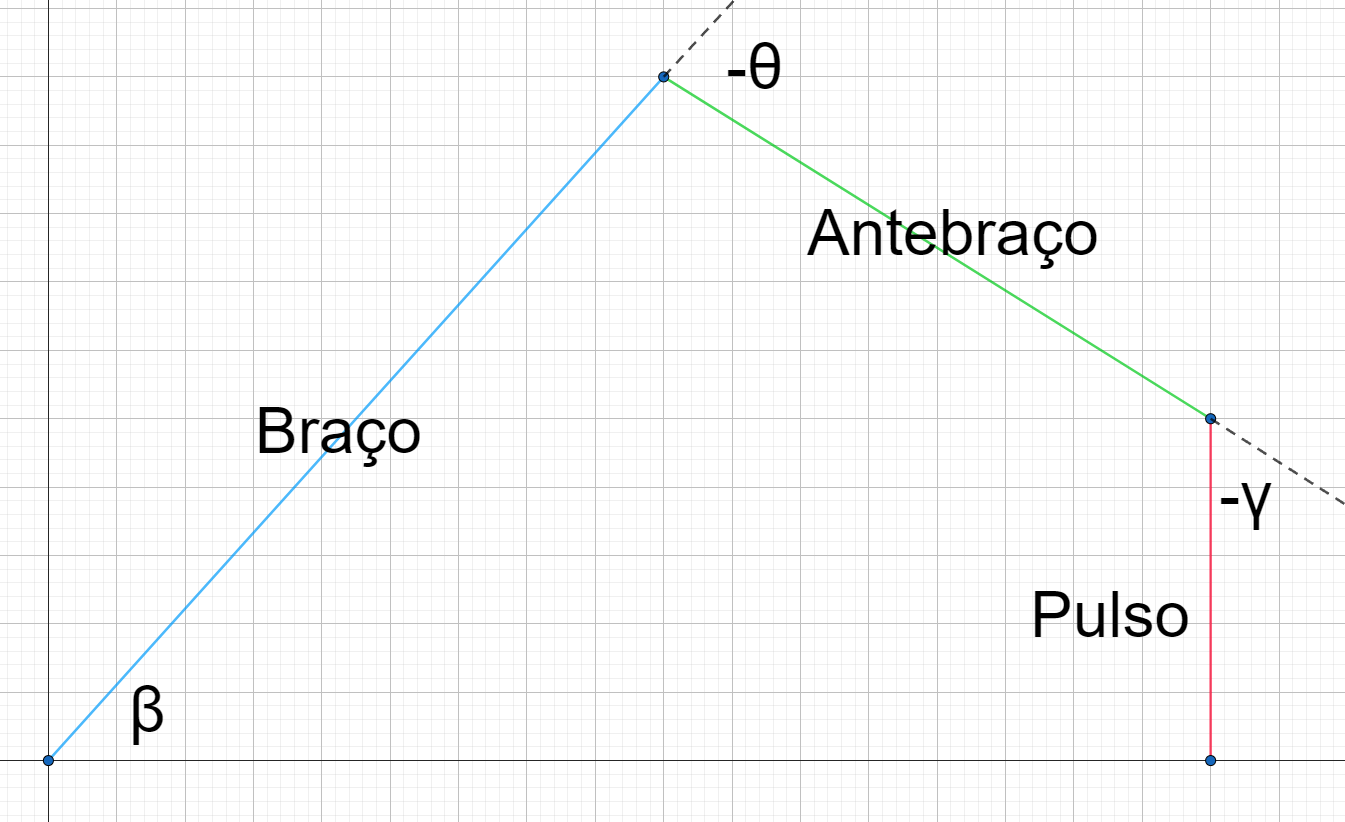
\includegraphics[keepaspectratio=true, width=0.7\textwidth]
    	{img/Cálculo ângulo pulso.png}
    \fonte{Do próprio autor}
    \label{fig:calculoAnguloPulso}
\end{figure}

Para facilitar a visualização dos ângulos e permitir uma comparação visual entre a posição desejada do manipulador e sua posição real,
foi desenvolvido um simples \textit{script} em Python que implementa um modelo simplificado do manipulador.
Esse \textit{script} permite movimentar o modelo para uma determinada posição \textit{x}, \textit{y} e \textit{z}, e exibe os ângulos calculados para cada junta.
A Figura \ref{fig:modeloManipulador} mostra o modelo desenvolvido.

\begin{figure}[H]
    \centering
    \caption{Modelo simplificado do manipulador}
    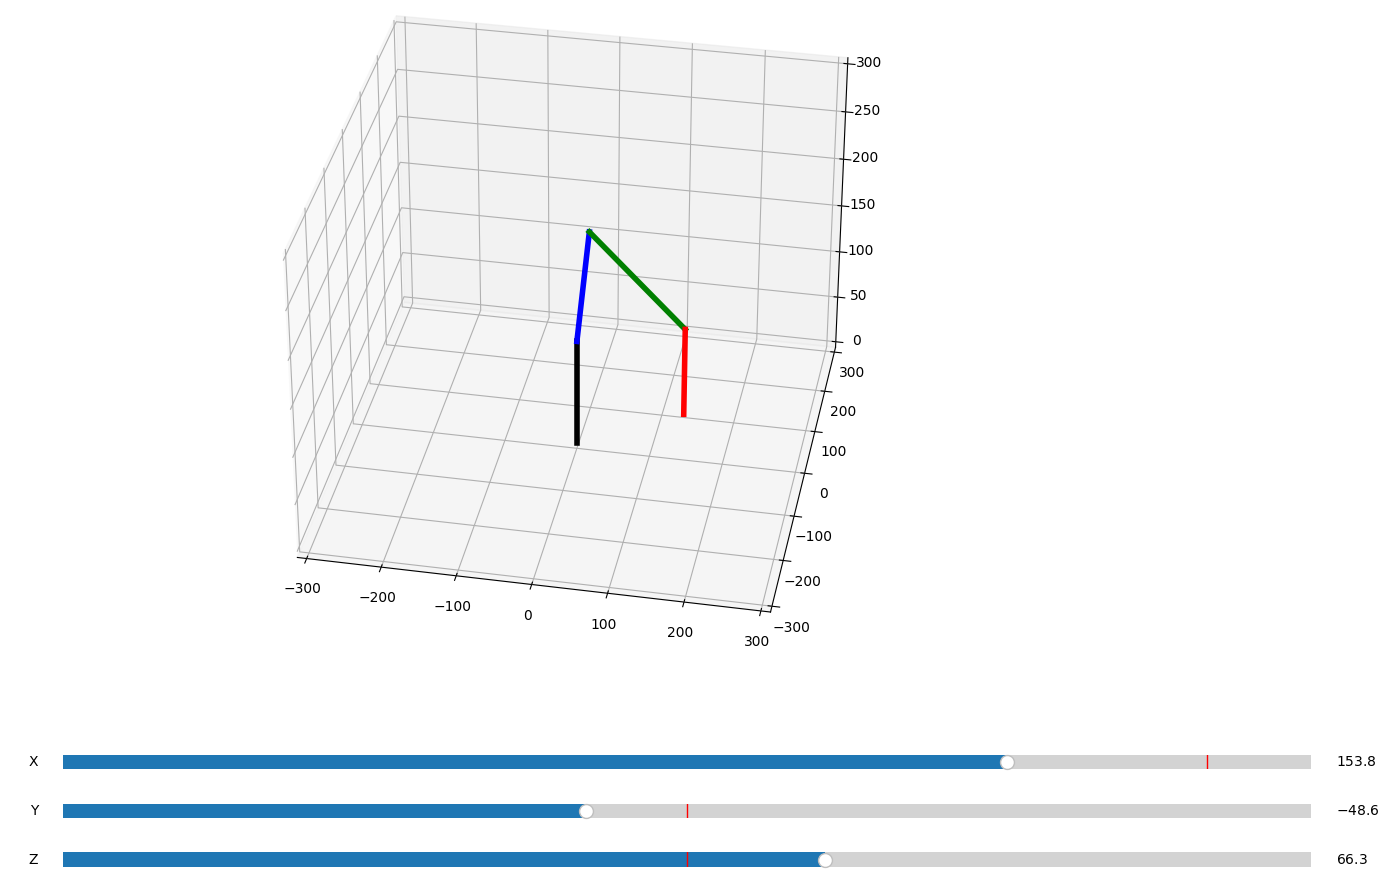
\includegraphics[keepaspectratio=true, width=1\textwidth]
    	{img/modelo-manipulador.png}
    \fonte{Do próprio autor}
    \label{fig:modeloManipulador}
\end{figure}

\section[Movimentação de peças]{Movimentação de peças}
\label{sec:movimentacaoPecas}

Depois de desenvolvida a funcionalidade de cálculo dos ângulos para movimentar o manipulador para uma determinada posição, foi necessário adicionar uma funcionalidade para utilizar o manipulador para pegar, mover e soltar as peças de xadrez.

Para isso, foi primeiramente definido de forma prática uma altura de movimentação do manipulador, que permite que ele mova livremente sem derrubar nenhuma peça e 
uma altura para pegar as peças, na qual a garra consegue alcançar e pegar qualquer peça.
Em seguida, foram mapeadas as coordenadas \textit{x} e \textit{y} de todas as casas do tabuleiro. Devido à uma limitação no tamanho do manipulador utilizado, não foi possível alcançar algumas casas, portanto as peças nessas casas devem ser movimentadas manualmente pelo jogador.

A partir disso, foi implementada uma funcionalidade para movimentar o manipulador para uma determinada casa do tabuleiro, apenas nos eixos \textit{x} e \textit{y}.
Em seguida, foi adicionada uma funcionalidade para pegar e outra para soltar a peça que está na casa atual do manipulador, movimentando-o apenas no eixo \textit{z} e acionando a garra.
Por fim, foi feita uma funcionalidade para movimentar o manipulador para a posição de repouso e outra para movimentá-lo para a posição de descarte de peças.

Devido à relação não linear entre os ângulos das juntas e a posição do manipulador,
foi observado que o manipulador não se movimentava adequadamente entre as casas do tabuleiro,
frequentemente derrubando peças.
Para solucionar esse problema, cada movimento do manipulador foi dividido em diversos movimentos menores,
de forma que o manipulador se movimente de forma mais suave e controlada.

\section[Comunicação com o computador]{Comunicação com o computador}
\label{sec:comunicacaoComputador}

Após finalizar a movimentação das peças, foi desenvolvido o módulo responsável por realizar a comunicação entre o microcontrolador e o computador.

Conforme descrito na subseção \ref{sub:computador}, essa comunicação é feita via protocolo serial, por meio de um cabo USB.
Entretanto, ainda era necessário definir o formato dos dados que serão enviados e recebidos.

Para isso, foram definidos alguns comandos que podem ser enviados pelo computador para o microcontrolador, conforme descrito na Tabela \ref{tab:comandosMicrocontrolador}.

\begin{table}[H]
    \centering
    \caption{Comandos enviados pelo computador para o microcontrolador}
    \begin{tabular}{|c|c|c|}
        \hline
        \textbf{Comando} & \textbf{Descrição} & \textbf{Formato} \\
        \hline
        move & Movimentar para casa & move \textit{x} \textit{y} \\
        \hline
        grab & Pegar peça & grab \\
        \hline
        release & Soltar peça & release \\
        \hline
        discard & Movimentar para posição de descarte & discard \\
        \hline
        reset & Movimentar para posição de repouso & reset \\
        \hline
        wait & Aguarde por \textit{n} milisegundos & wait \textit{n} \\
        \hline
    \end{tabular}
    \fonte{Do próprio autor}
    \label{tab:comandosMicrocontrolador}
\end{table}

Ao final da execução de cada comando, o microcontrolador envia uma mensagem de confirmação para o computador, informando se o comando foi executado com sucesso (OK) ou não (FAIL).

Para possibilitar o controle manual do manipulador, foram definidas algumas mensagens que podem ser enviadas pelo microcontrolador para o computador, conforme descrito na Tabela \ref{tab:mensagensMicrocontrolador}.

\begin{table}[H]
    \centering
    \caption{Mensagens enviadas pelo microcontrolador para o computador}
    \begin{tabular}{|c|c|c|}
        \hline
        \textbf{Mensagem} & \textbf{Descrição} & \textbf{Formato} \\
        \hline
        joystick & \textit{Joystick} foi movimentado & joystick <up down left right> \\
        \hline
        select & Botão do \textit{joystick} foi pressionado & select \\
        \hline
    \end{tabular}
    \fonte{Do próprio autor}
    \label{tab:mensagensMicrocontrolador}
\end{table}

\section[Implementação da lógica de xadrez]{Implementação da lógica de xadrez}
\label{sec:implementacaoLogicaXadrez}

Depois de finalizar a comunicação entre o microcontrolador e o computador, foi desenvolvido o \textit{software} responsável por implementar a lógica do jogo de xadrez.

O \textit{software} foi desenvolvido em Python, utilizando a biblioteca \textit{stockfish} \cite{stockfish_python} para realizar comunicação com a \textit{engine} de xadrez \textit{Stockfish} 15.1 \cite{stockfish_engine}.
Essa \textit{engine} é responsável por verificar quais movimentos são válidos e calcular qual movimento o computador deve jogar em cada turno.

Além da utilização da biblioteca \textit{stockfish}, foi necessário implementar algumas funcionalidades manualmente que não existem nela.
Em primeiro lugar, foi implementada uma função para adquirir quais movimentos são válidos para a posição atual do tabuleiro, utilizando o comando \textit{go perft 1} da \textit{engine} \textit{Stockfish}.
Em seguida, foi desenvolvida uma funcionalidade para detectar quando a partida acabou, verificando se não existe mais nenhum movimento válido para o jogador atual.
Por último, foi feita uma função para verificar se o jogo terminou empatado, verificando a avaliação da posição atual do tabuleiro pela \textit{engine} \textit{Stockfish}.

Para comunicar com o microcontrolador, foi utilizada a biblioteca PySerial \cite{pyserial}.
Através dessa biblioteca, é possível enviar e receber as mensagens descritas na seção \ref{sec:comunicacaoComputador}.
Após enviar uma mensagem para o microcontrolador, o \textit{software} aguarda uma mensagem de confirmação para indicar o sucesso ou falha da execução do comando.

Ao iniciar uma partida, o programa exibe uma mensagem para o usuário escolher qual modo de jogo deseja utilizar: jogar contra o computador ou contra outra pessoa.
No primeiro modo, o \textit{software} \textit{Stockfish} 15.1 é utilizado para calcular qual movimento o computador irá jogar, 
enquanto no segundo modo, o jogador que estiver controlando o manipulador pode movimentá-lo pelas casas do tabuleiro e pegar peças sem restrição, entretanto ao tentar soltar uma peça, é feita uma consulta ao \textit{Stockfish} 15.1 para validar se a jogada desejada é válida.
Em ambos os modos de jogo, os movimentos realizados pelo jogador humano que não controla o manipulador robótico devem ser digitados manualmente no computador.

Em seguida, o programa exibe uma mensagem para o usuário escolher qual cor de peças deseja utilizar: brancas ou pretas.
Depois disso, caso o usuário tenha escolhido jogar contra o computador, o programa exibe uma mensagem para o usuário escolher qual nível de dificuldade deseja utilizar.
Esse nível pode variar de 1 a 20, sendo 1 o nível mais fácil e 20 o nível mais difícil.
Por fim, o programa inicia a partida e exibe o tabuleiro atualizado a cada jogada, conforme ilustrado na Figura \ref{fig:softwareTabuleiro}.
O usuário deve digitar o movimento que deseja realizar no formato \textit{<casa de origem><casa de destino>}, por exemplo \textit{e2e4} para mover o peão da casa \textit{e2} para a casa \textit{e4}.

\begin{figure}[H]
    \centering
    \caption{Tela do programa mostrando o tabuleiro atualizado}
    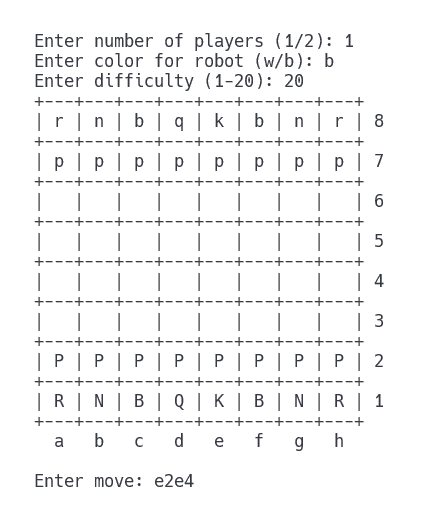
\includegraphics[keepaspectratio=true, width=0.5\textwidth]
    	{img/software-tabuleiro.png}
    \fonte{Do próprio autor}
    \label{fig:softwareTabuleiro}
\end{figure}

Ao detectar uma captura de peça, o programa primeiro controla o manipulador para movimentar a peça capturada para a posição de descarte.
Em seguida é feita a movimentação da peça que capturou para a casa de destino.
Foi feito um tratamento especial para capturas do tipo \textit{en passant}, pois nesses movimentos a peça capturada não está na casa de destino.
Nesse caso, a casa do peão capturado pode ser obtido através da linha da peça capturadora e da coluna da casa de destino.

Um outro tratamento especial foi feito para movimentos de roque, pois nesses movimentos duas peças são movimentadas ao mesmo tempo.
Nesse caso, o manipulador primeiro movimenta o rei para a casa de destino e em seguida movimenta a torre para a casa de destino.

Por fim, caso o manipulador robótico esteja jogando com as peças pretas,
o programa realiza uma conversão da posição do tabuleiro para realizar o movimento adequado.
Nesse caso, o tabuleiro é invertido horizontalmente e verticalmente,
e as casas de origem e destino são convertidas para suas respectivas casas invertidas.
Dessa forma, o manipulador pode movimentar as peças pretas da mesma forma que movimenta as peças brancas.

A Figura \ref{fig:manipuladorRepouso} mostra o manipulador robótico em sua posição de repouso, aguardando o jogador humano realizar seu movimento.
Depois disso, o computador realiza seu movimento e o manipulador se movimenta para a casa de origem da peça que deseja movimentar, conforme ilustrado na Figura \ref{fig:manipuladorMovimentandoPosicao}.
Ao chegar na casa de origem, o manipulador se movimenta no eixo \textit{z} e pega a peça, como ilustrado na Figura \ref{fig:manipuladorPegandoPeça}.
Após pegar a peça, o manipulador se movimenta para a casa de destino, conforme ilustrado na Figura \ref{fig:manipuladorLevandoPeça}.
Em seguida, o manipulador se movimenta no eixo \textit{z} e solta a peça, como ilustrado na Figura \ref{fig:manipuladorSoltandoPeça}.
Por fim, a Figura \ref{fig:manipuladorRetornandoRepouso} mostra o manipulador retornando para sua posição de repouso, onde aguarda o próximo movimento do jogador humano.

\begin{figure}[H]
    \centering
    \caption{Manipulador robótico em posição de repouso}
    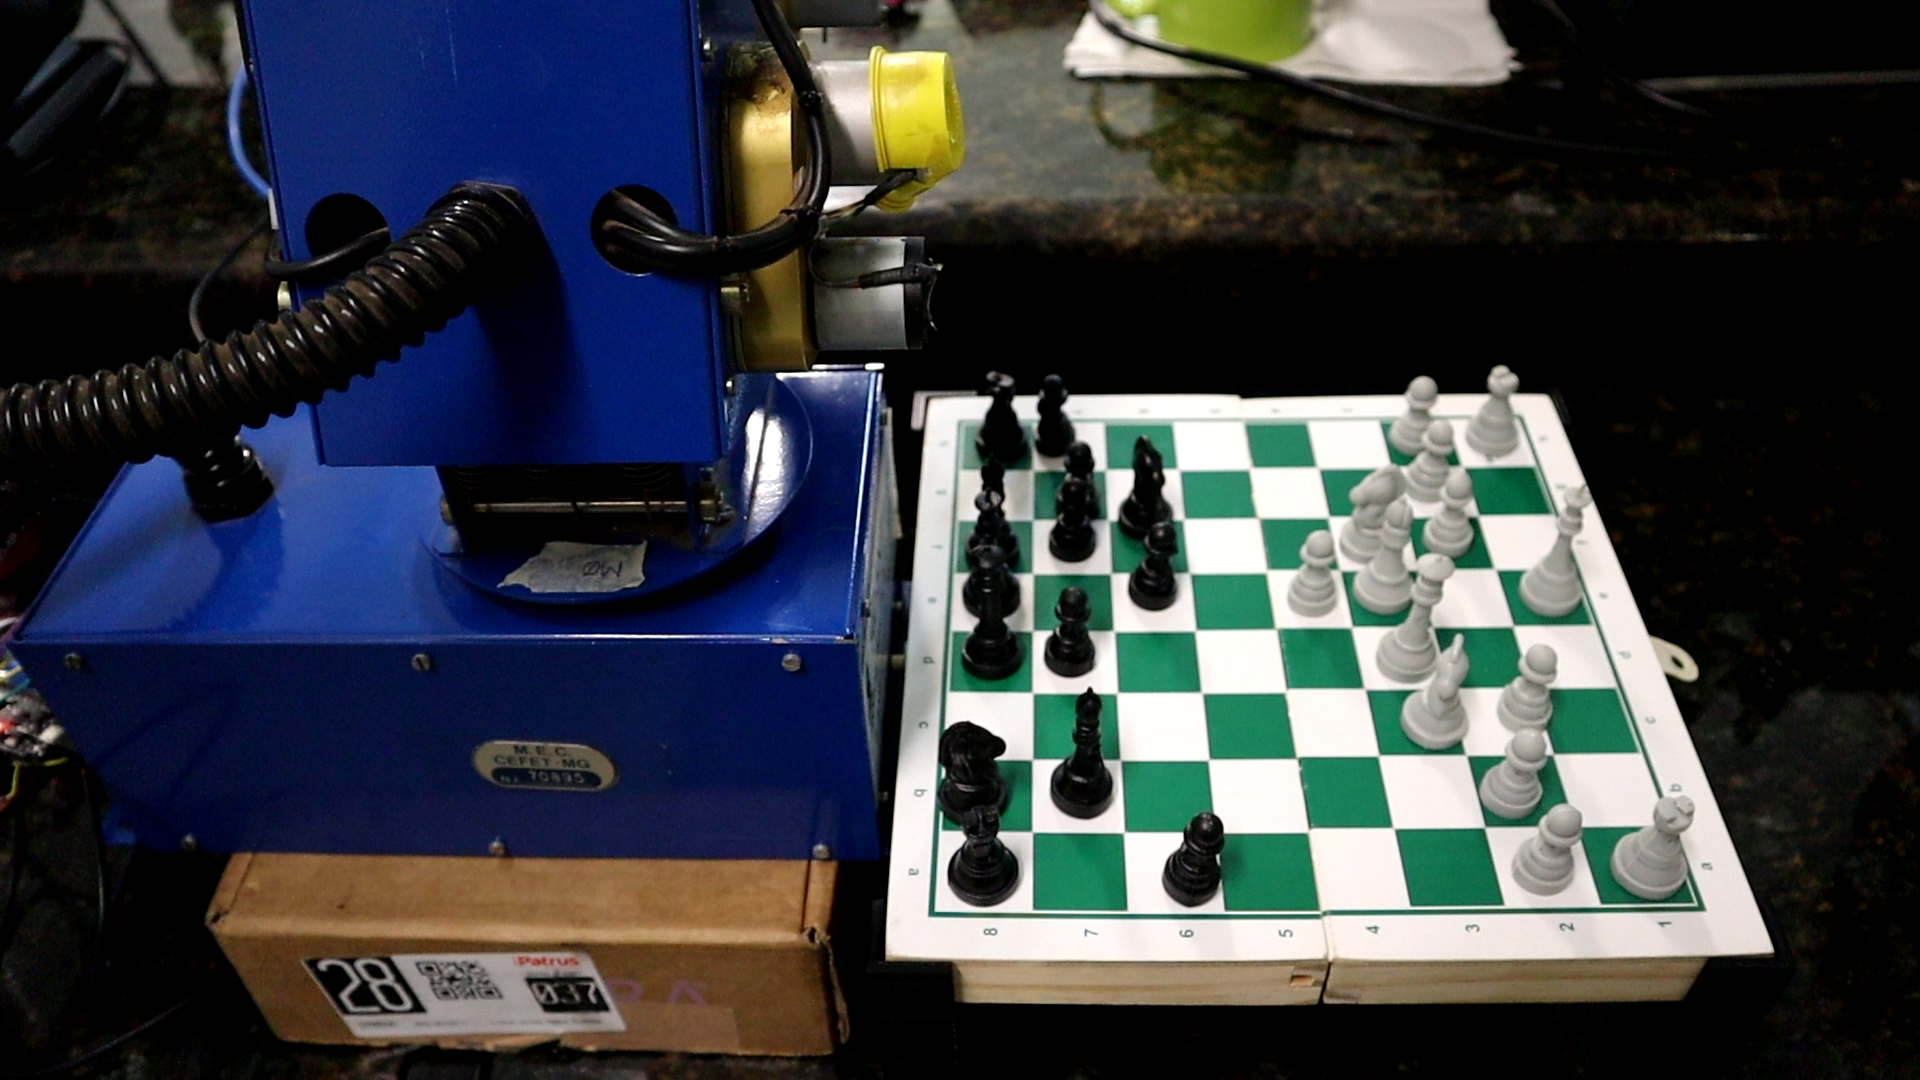
\includegraphics[keepaspectratio=true, width=0.9\textwidth]
    	{img/posicao-repouso.png}
    \fonte{Do próprio autor}
    \label{fig:manipuladorRepouso}
\end{figure}

\begin{figure}[H]
    \centering
    \caption{Manipulador robótico movimentando para a casa de origem}
    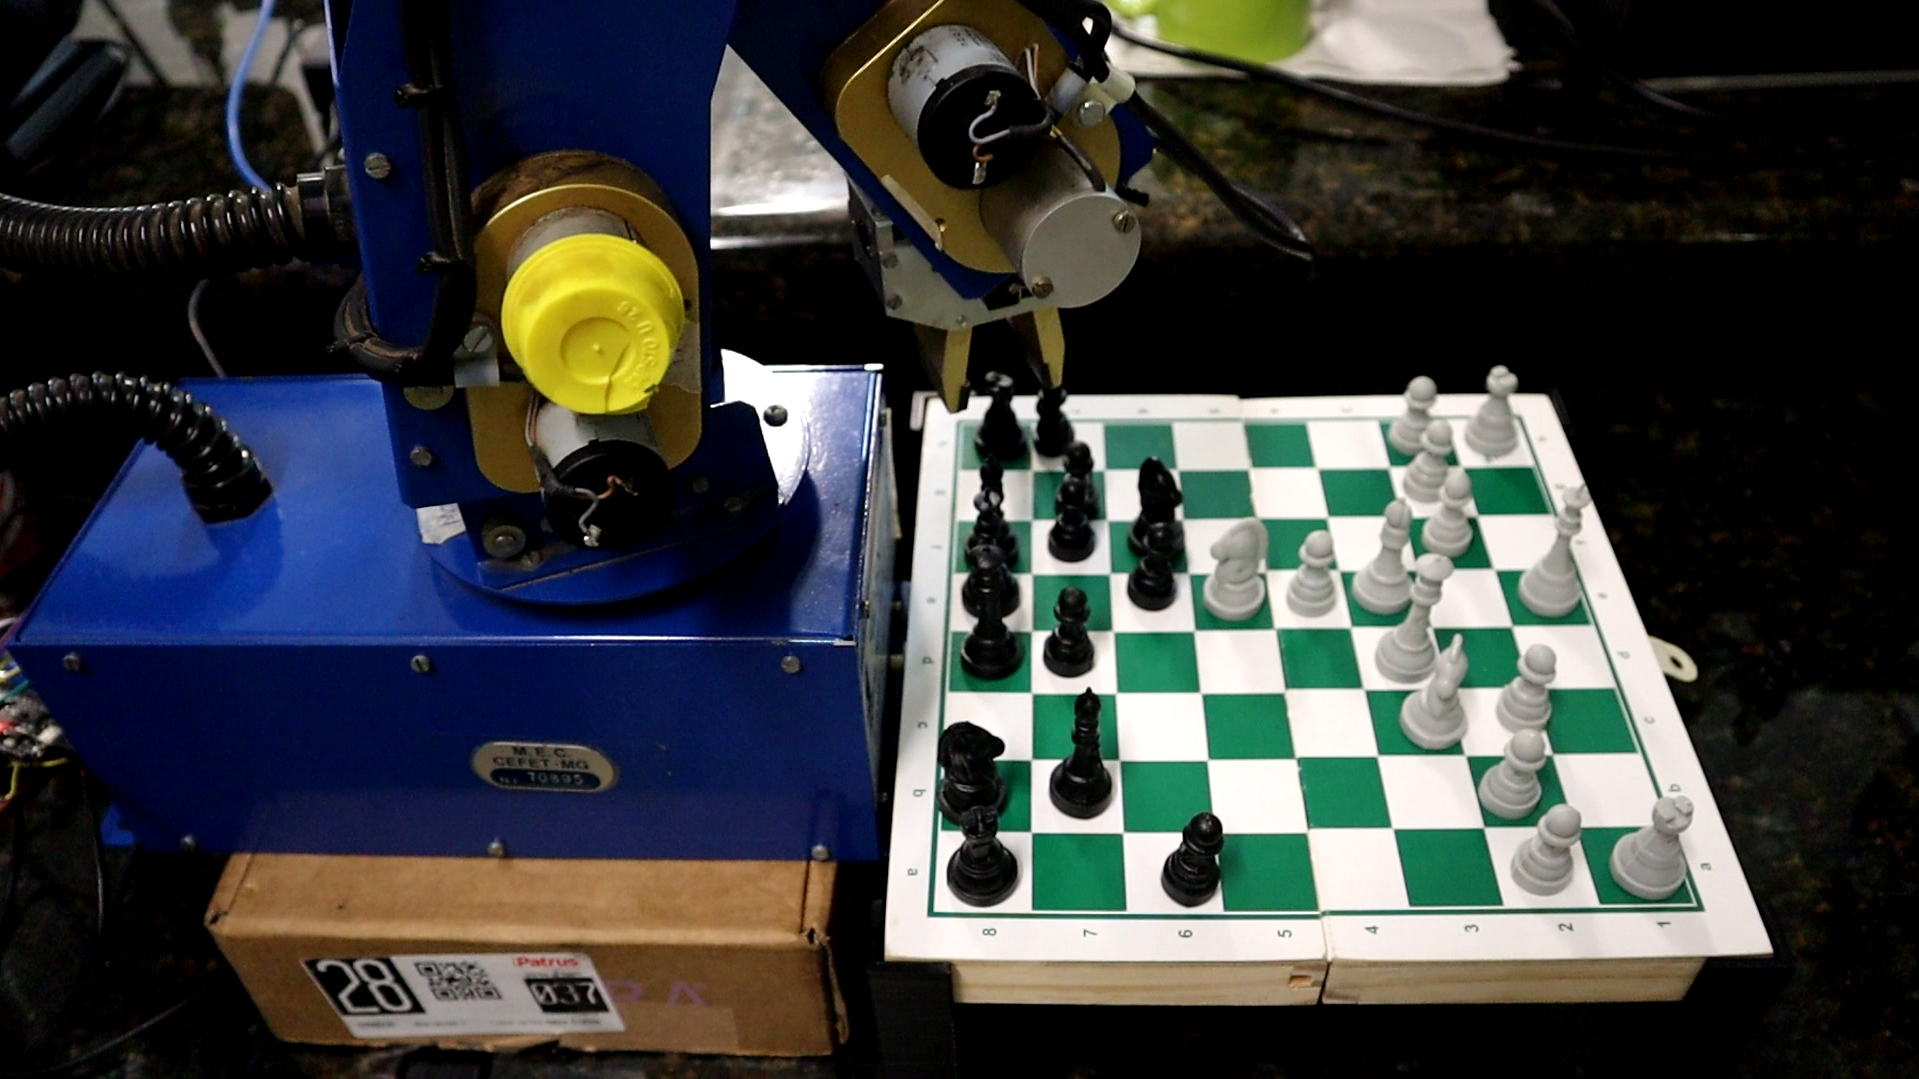
\includegraphics[keepaspectratio=true, width=0.9\textwidth]
    	{img/movimentando-posicao.png}
    \fonte{Do próprio autor}
    \label{fig:manipuladorMovimentandoPosicao}
\end{figure}

\begin{figure}[H]
    \centering
    \caption{Manipulador robótico pegando a peça}
    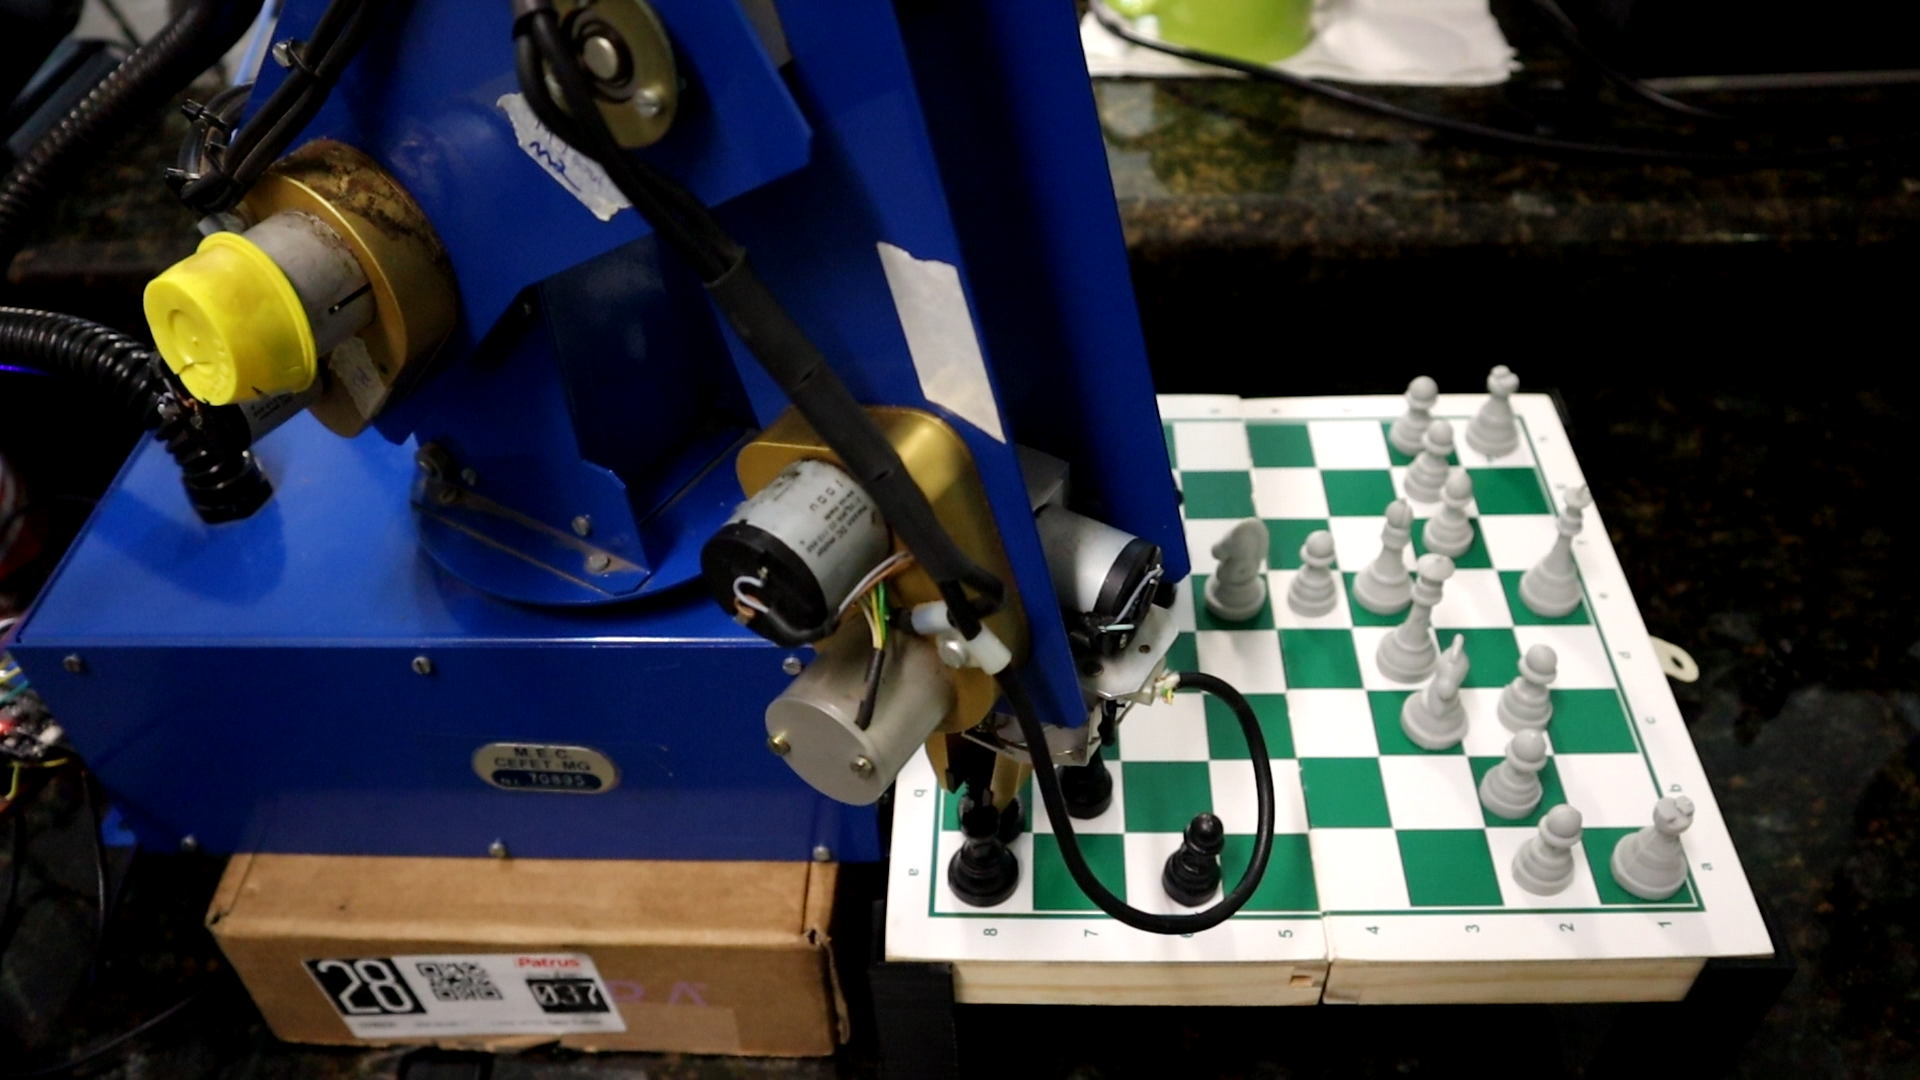
\includegraphics[keepaspectratio=true, width=0.9\textwidth]
    	{img/pegando-peca.png}
    \fonte{Do próprio autor}
    \label{fig:manipuladorPegandoPeça}
\end{figure}

\begin{figure}[H]
    \centering
    \caption{Manipulador robótico levando a peça para a casa de destino}
    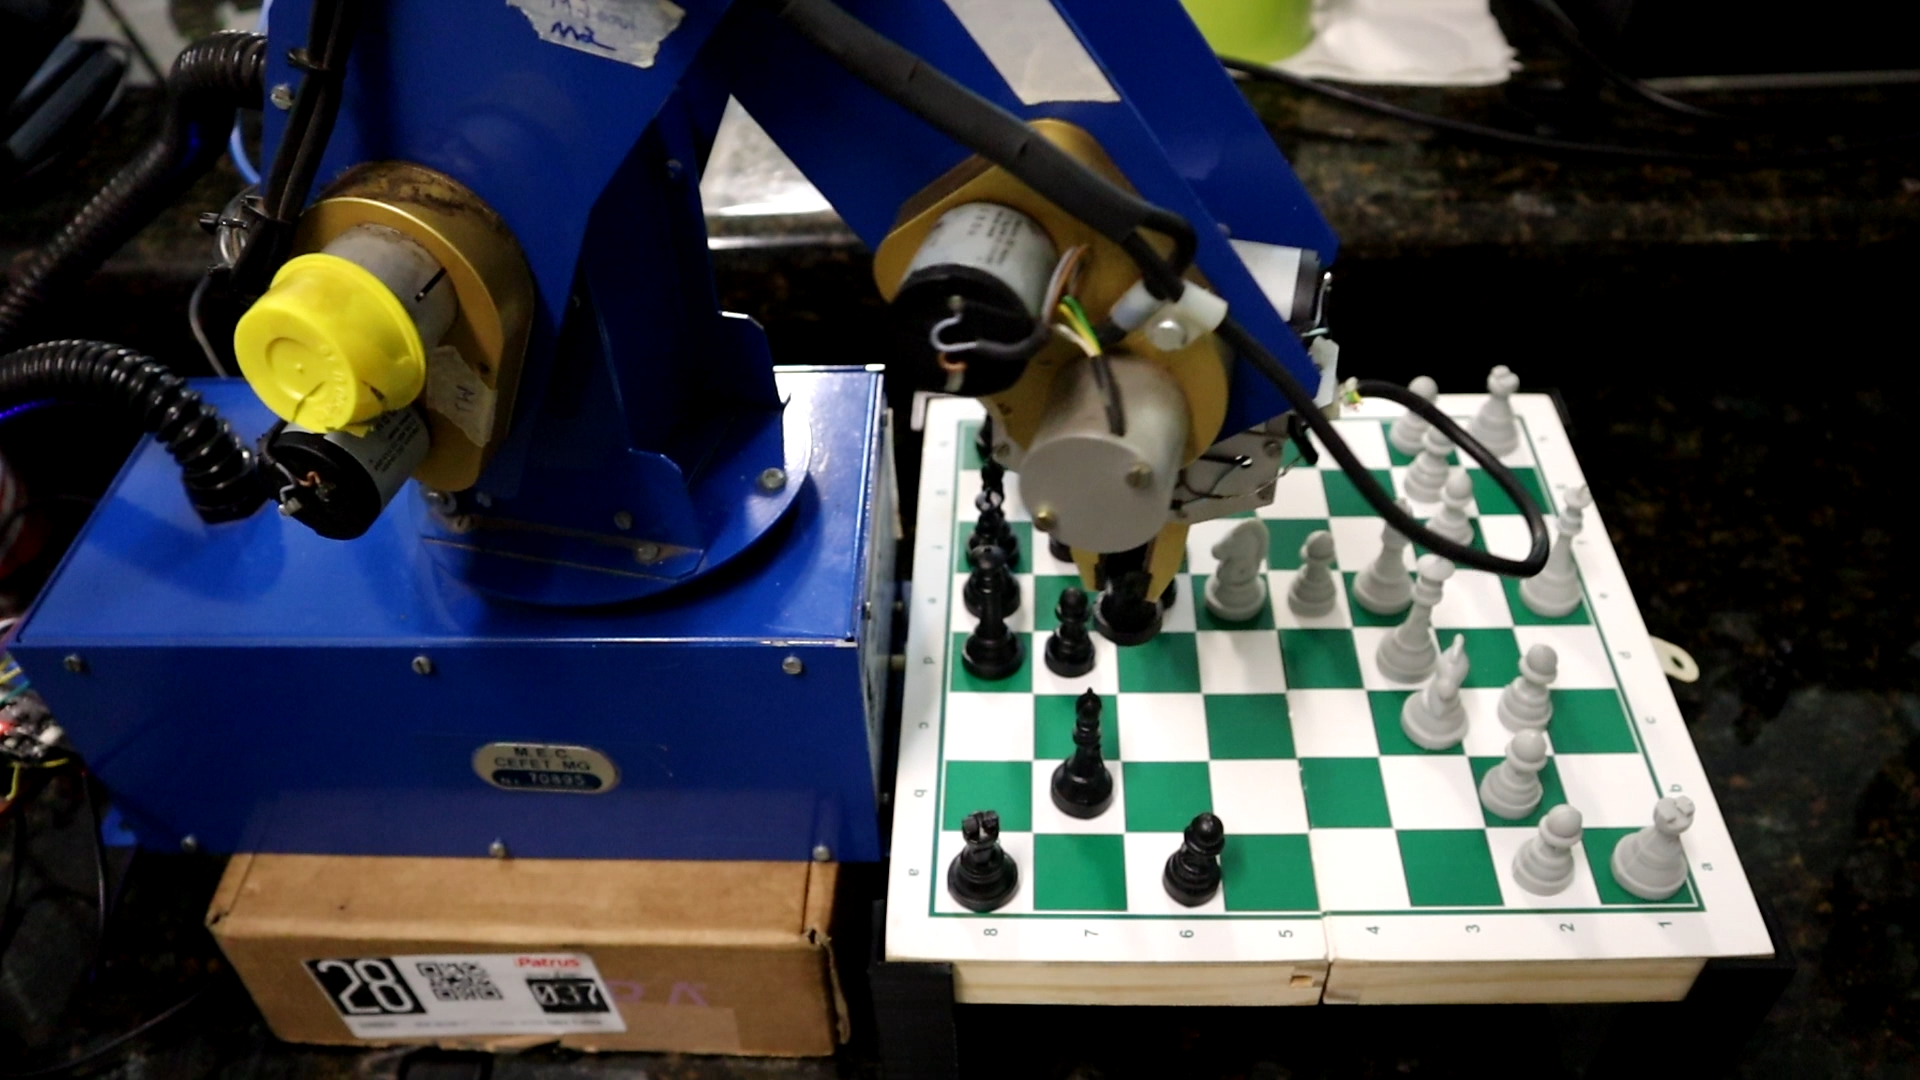
\includegraphics[keepaspectratio=true, width=0.9\textwidth]
    	{img/levando-peca.png}
    \fonte{Do próprio autor}
    \label{fig:manipuladorLevandoPeça}
\end{figure}

\begin{figure}[H]
    \centering
    \caption{Manipulador robótico soltando a peça}
    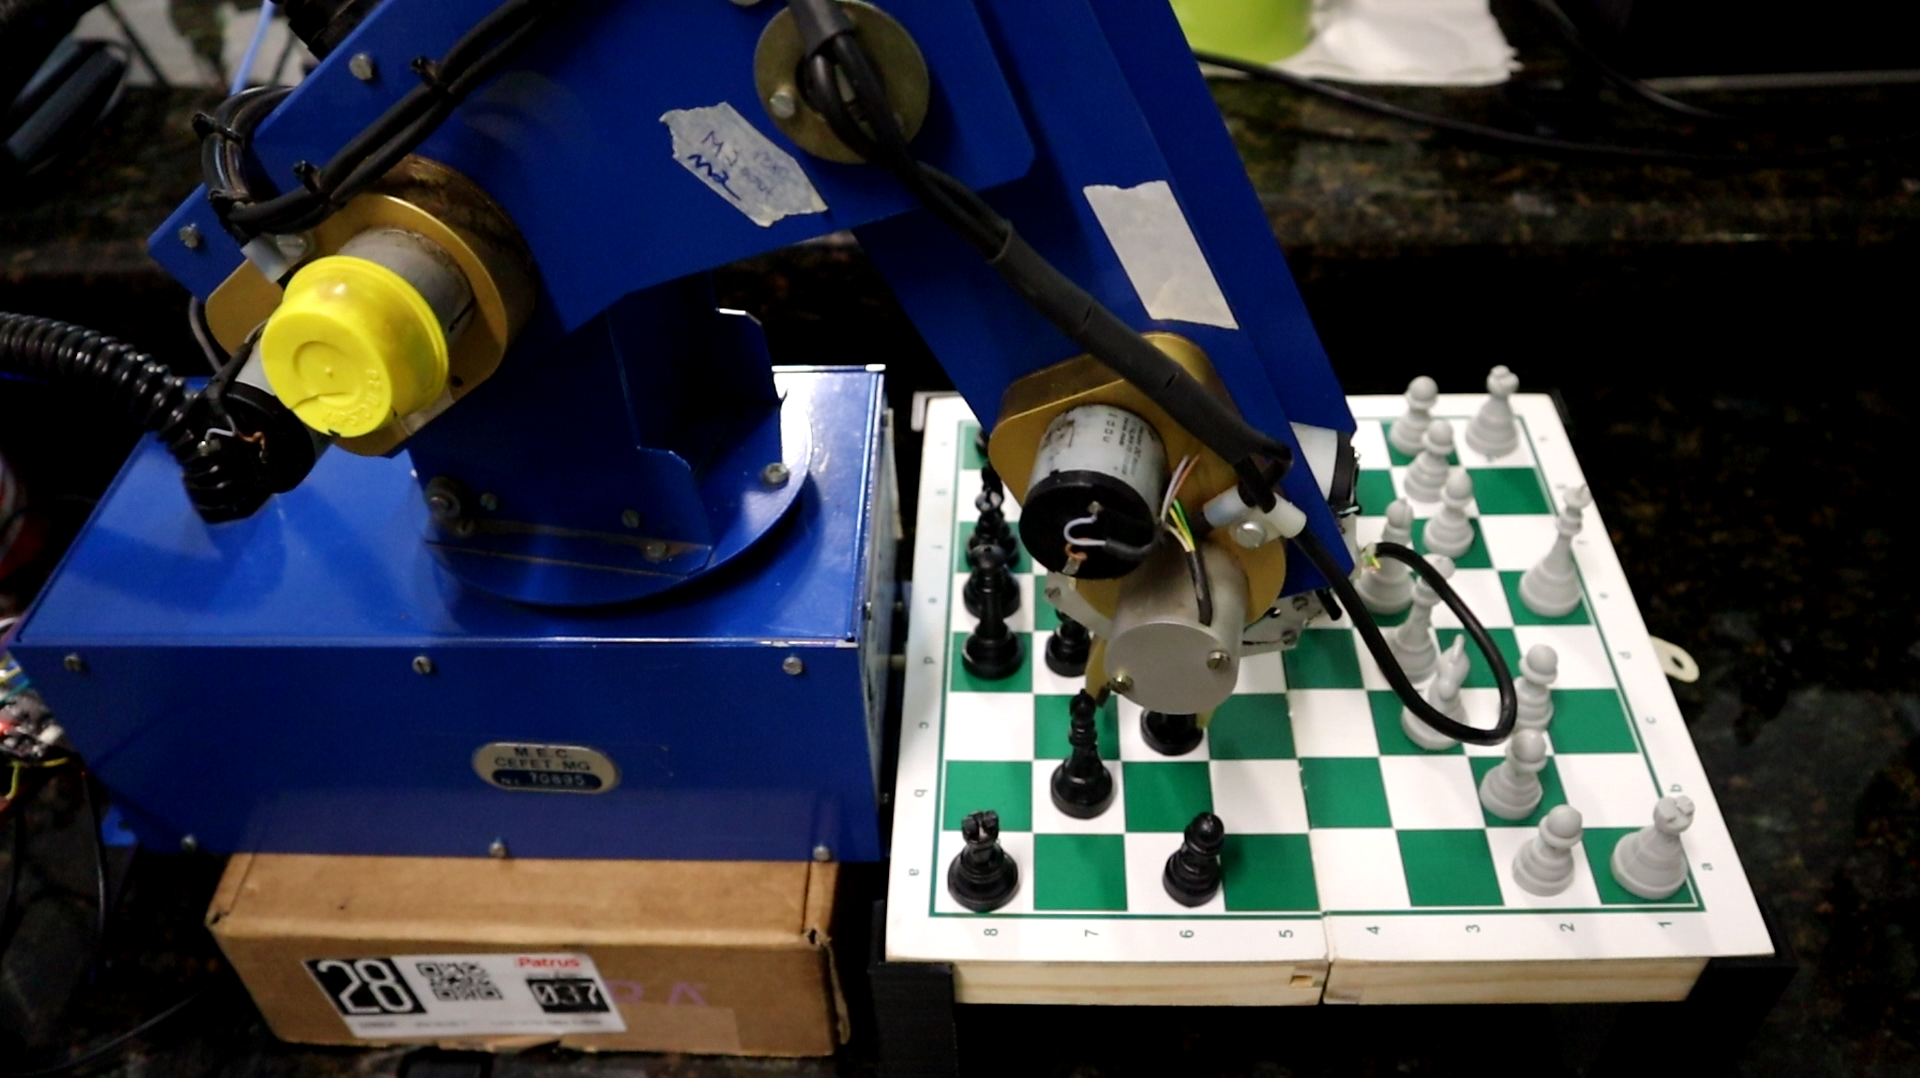
\includegraphics[keepaspectratio=true, width=0.9\textwidth]
    	{img/soltando-peca.png}
    \fonte{Do próprio autor}
    \label{fig:manipuladorSoltandoPeça}
\end{figure}

\begin{figure}[H]
    \centering
    \caption{Manipulador robótico retornando para a posição de repouso}
    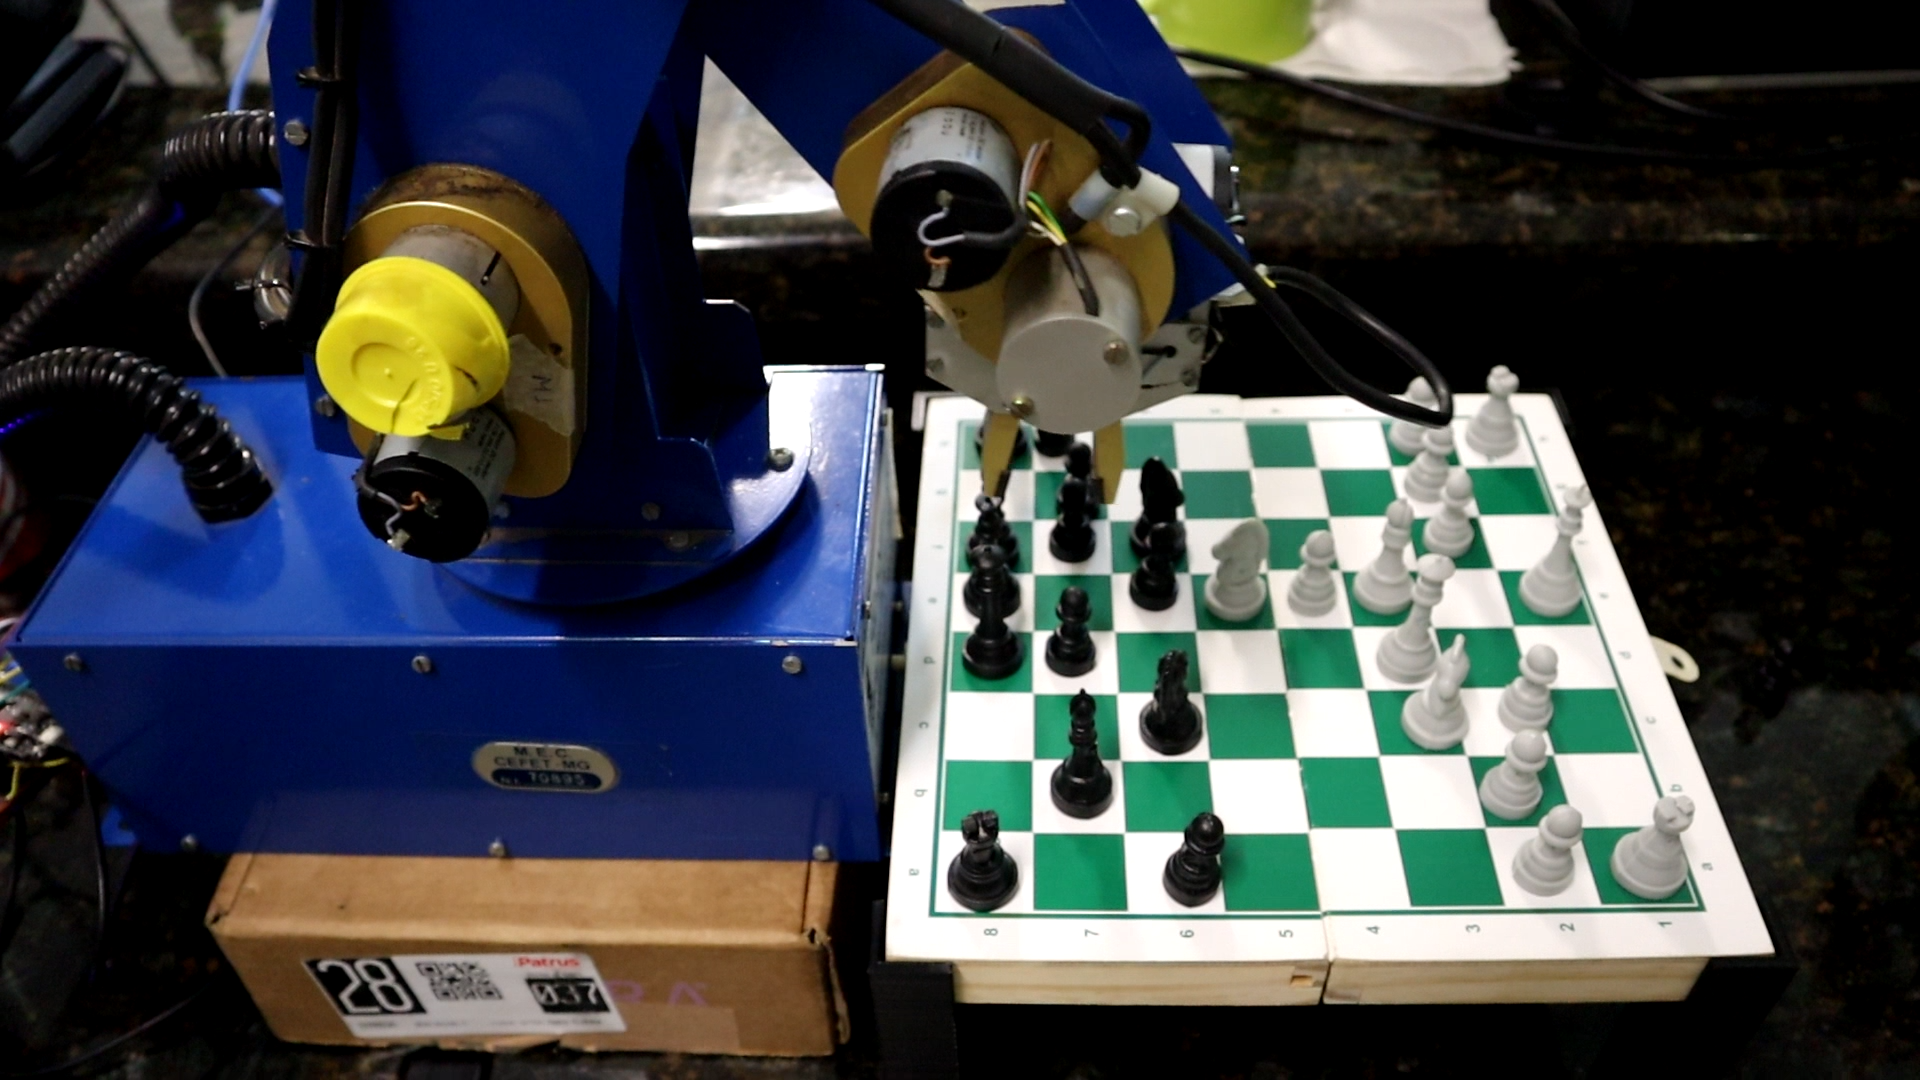
\includegraphics[keepaspectratio=true, width=0.9\textwidth]
    	{img/retornando-repouso.png}
    \fonte{Do próprio autor}
    \label{fig:manipuladorRetornandoRepouso}
\end{figure}

\section[Análise de Desempenho]{Análise de Desempenho}
\label{sec:implementacaoLogicaXadrez}

Depois de finalizado o desenvolvimento do sistema, foi feita uma análise de sua performance,
com o objetivo de verificar quanto tempo o manipulador robótico leva para realizar um movimento.

Para isso, foi jogada uma partida contra o computador, anotando o tempo gasto para cada movimento realizado pelo manipulador robótico.
O resultados obtidos estão apresentados na Tabela \ref{tab:performance},
utilizando a notação algébrica descrita na Subseção \ref{sub:xadrezNotacao}.
O vídeo dessa partida pode ser acessado no link \url{https://youtu.be/6tGpsd19aSE}.

\begin{table}[H]
    \centering
    \caption{Tempo de execução de cada movimento}
    \label{tab:performance}
    \begin{tabular}{|c|c|c|c|}
        \hline
        & \textbf{Humano} & \textbf{Computador} & \textbf{Tempo (s)} \\
        \hline
        1 & e4 & c5 & 20.7 \\
        \hline
        2 & Nf3 & e6 & 19.0 \\
        \hline
        3 & Nc3 & a6 & 23.2 \\
        \hline
        4 & Bc4 & b5 & 21.5 \\
        \hline
        5 & Bb3 & c4 & 20.9 \\
        \hline
        6 & Bxc4 & bxc4 & 41.8 \\
        \hline
        7 & d3 & cxd3 & 41.8 \\
        \hline
        8 & Qxd3 & Bb7 & 21.6 \\
        \hline
        9 & Be3 & Nf6 & 18.8 \\
        \hline
        10 & Ne5 & Nc6 & 21.2 \\
        \hline
        11 & O-O & Nxe5 & 40.0 \\
        \hline
        12 & Qe2 & Qc7 & 19.8 \\
        \hline
        13 & f3 & Bc5 & 19.8 \\
        \hline
        14 & Bxc5 & Qxc5+ & 41.4 \\
        \hline
        \multicolumn{3}{|c|}{\textbf{Tempo médio}} & 26.5 \\
        \hline
        \multicolumn{3}{|c|}{\textbf{Tempo médio movimento}} & 20.7 \\
        \hline
        \multicolumn{3}{|c|}{\textbf{Tempo médio captura}} & 41.3 \\
        \hline
    \end{tabular}
\end{table}

Como pode ser observado na Tabela \ref{tab:performance}, o manipulador gasta em torno de 21 segundos para movimentar uma peça.
Movimentos de captura requerem a movimentação de duas peças, portanto gastam o dobro do tempo.
Esse tempo é relativamente alto para um jogo competitivo de xadrez, entretanto é adequado para o objetivo proposto neste trabalho.

\chapter[Conclusão]{Conclusão}
\label{cap:conclusao}

A partir do desenvolvimento deste trabalho, foi possível obter uma plataforma simples e de baixo custo que permite o jogo entre duas pessoas ou entre uma pessoa e o computador.
Essa plataforma pode ser apresentada para crianças e jovens em feiras e eventos para introduzir conceitos básicos de computação, engenharia elétrica e controle de sistemas, além de instigar o conhecimento nessas áreas.

\section[Limitações]{Limitações}
\label{sec:limitacoes}

O projeto apresenta algumas limitações que podem ser melhoradas em trabalhos futuros.

Em primeiro lugar, o manipulador robótico escolhido não apresenta tamanho suficiente para alcançar todas as casas do tabuleiro,
o que limita o jogo, principalmente quando uma pessoa está controlando o dispositivo.
A escolha de um modelo de manipulador robótico com maior alcance pode resolver esse problema.

Além disso, o projeto não apresenta um sistema de detecção de peças no tabuleiro,
o que faz com que o usuário tenha que informar ao computador qual peça foi movida.
A implementação de um sistema de visão computacional pode tornar o sistema muito mais interativo e intuitivo.

Por fim, o controle do manipulador não é muito preciso, o que pode causar erros na movimentação das peças.
Em algumas situações, o manipulador pode derrubar uma peça ao tentar movimentá-la.
A implementação de um sistema de controle mais robusto pode resolver esse problema e evitar que erros aconteçam durante a movimentação.
Também é possível implementar um sistema de detecção de erros durante a movimentação das peças utilizando visão computacional.

% ----------------------------------------------------------








% ----------------------------------------------------------
% Finaliza a parte no bookmark do PDF
% para que se inicie o bookmark na raiz
% e adiciona espaço de parte no Sumário
% ----------------------------------------------------------
\phantompart







% ----------------------------------------------------------
% ELEMENTOS PÓS-TEXTUAIS
% ----------------------------------------------------------

%% Baseado no arquivo: 
%% abtex2-modelo-trabalho-academico.tex, v-1.9.6 laurocesar
%% by abnTeX2 group at http://www.abntex.net.br/ 
%% Adaptado para um modelo de TCC (Graduação)

\postextual
% ----------------------------------------------------------

% ----------------------------------------------------------
% Referências bibliográficas
% ----------------------------------------------------------
\bibliography{cefet_mg_decom_abntex2}

% ----------------------------------------------------------
% Glossário
% ----------------------------------------------------------
%
% Consulte o manual da classe abntex2 para orientações sobre o glossário.
%
%\glossary

% ----------------------------------------------------------
% Apêndices
% ----------------------------------------------------------

% ---
% Inicia os apêndices
% ---
\begin{apendicesenv}

% Imprime uma página indicando o início dos apêndices
\partapendices

% ----------------------------------------------------------
\chapter{Título do primeiro apêndice}
% ----------------------------------------------------------

Suspendisse sollicitudin risus et accumsan tempor. Orci varius natoque penatibus et magnis dis parturient montes, nascetur ridiculus mus. Mauris tempor malesuada ligula sed vehicula. Fusce porta magna a blandit aliquet. Nullam auctor tellus et augue lobortis suscipit. Nunc aliquet interdum nisl, at accumsan ante. Donec convallis arcu massa, eu malesuada ex tincidunt quis. Suspendisse turpis orci, auctor et egestas sit amet, ultrices a nisl. Ut interdum metus eu erat facilisis cursus. Maecenas sed dignissim odio, non tempor ipsum. Quisque luctus mi non molestie volutpat.

Class aptent taciti sociosqu ad litora torquent per conubia nostra, per inceptos himenaeos. Proin sed nulla auctor, tempor mauris nec, placerat justo. Vestibulum finibus aliquet ultricies. Nulla facilisi. Ut ante orci, interdum ac sodales vel, porttitor eu justo. Proin laoreet lacinia sapien, non suscipit libero bibendum sit amet. 

% ----------------------------------------------------------
\chapter{Outro Apêndice}
% ----------------------------------------------------------
Nulla facilisi. Ut ante orci, interdum ac sodales vel, porttitor eu justo. Proin laoreet lacinia sapien, non suscipit libero bibendum sit amet. Aliquam orci risus, venenatis et nibh eget, dictum imperdiet ligula. Suspendisse sollicitudin risus et accumsan tempor. Orci varius natoque penatibus et magnis dis parturient montes, nascetur ridiculus mus. Mauris tempor malesuada ligula sed vehicula. Fusce porta magna a blandit aliquet. Nullam auctor tellus et augue lobortis suscipit. Nunc aliquet interdum nisl, at accumsan ante. Donec convallis arcu massa, eu malesuada ex tincidunt quis. Suspendisse turpis orci, auctor et egestas sit amet, ultrices a nisl. Ut interdum metus eu erat facilisis cursus. Maecenas sed dignissim odio, non tempor ipsum. Quisque luctus mi non molestie volutpat.

Nulla facilisi. Ut ante orci, interdum ac sodales vel, porttitor eu justo. Proin laoreet lacinia sapien, non suscipit libero bibendum sit amet.Mauris dictum ante urna, at posuere nulla fermentum id. Proin fermentum odio at elit tristique faucibus. Praesent sit amet facilisis enim, id pulvinar quam. Sed dignissim sem quis tortor tincidunt, mattis blandit eros viverra. Class aptent taciti sociosqu ad litora torquent per conubia nostra, per inceptos himenaeos. Proin sed nulla auctor, tempor mauris nec, placerat justo. Vestibulum finibus aliquet ultricies.  

\end{apendicesenv}
% ---


% ----------------------------------------------------------
% Anexos
% ----------------------------------------------------------

% ---
% Inicia os anexos
% ---
\begin{anexosenv}

% Imprime uma página indicando o início dos anexos
\partanexos

% ---
\chapter{Este é o título do primeiro anexo}
% ---
 Lorem ipsum dolor sit amet, consectetur adipiscing elit. Cras a ultrices dolor. Pellentesque id ex neque. Aliquam orci risus, venenatis et nibh eget, dictum imperdiet ligula. Suspendisse sollicitudin risus et accumsan tempor. Orci varius natoque penatibus et magnis dis parturient montes, nascetur ridiculus mus. Mauris tempor malesuada ligula sed vehicula. Fusce porta magna a blandit aliquet. Nullam auctor tellus et augue lobortis suscipit. Nunc aliquet interdum nisl, at accumsan ante. Donec convallis arcu massa, eu malesuada ex tincidunt quis. Suspendisse turpis orci, auctor et egestas sit amet, ultrices a nisl. Ut interdum metus eu erat facilisis cursus. Maecenas sed dignissim odio, non tempor ipsum. Quisque luctus mi non molestie volutpat.

Mauris dictum ante urna, at posuere nulla fermentum id. Proin fermentum odio at elit tristique faucibus. Praesent sit amet facilisis enim, id pulvinar quam. Sed dignissim sem quis tortor tincidunt, mattis blandit eros viverra. Class aptent taciti sociosqu ad litora torquent per conubia nostra, per inceptos himenaeos. Proin sed nulla auctor, tempor mauris nec, placerat justo. Vestibulum finibus aliquet ultricies. Nulla facilisi. Ut ante orci, interdum ac sodales vel, porttitor eu justo. Proin laoreet lacinia sapien, non suscipit libero bibendum sit amet. 

% ---
\chapter{SEgundo título do segundo anexo}
% ---
Aliquam orci risus, venenatis et nibh eget, dictum imperdiet ligula. Suspendisse sollicitudin risus et accumsan tempor. Orci varius natoque penatibus et magnis dis parturient montes, nascetur ridiculus mus. Mauris tempor malesuada ligula sed vehicula. Fusce porta magna a blandit aliquet. Nullam auctor tellus et augue lobortis suscipit. Nunc aliquet interdum nisl, at accumsan ante. Donec convallis arcu massa, eu malesuada ex tincidunt quis. Suspendisse turpis orci, auctor et egestas sit amet, ultrices a nisl. Ut interdum metus eu erat facilisis cursus. Maecenas sed dignissim odio, non tempor ipsum. Quisque luctus mi non molestie volutpat.

Praesent sit amet facilisis enim, id pulvinar quam. Sed dignissim sem quis tortor tincidunt, mattis blandit eros viverra. Class aptent taciti sociosqu ad litora torquent per conubia nostra, per inceptos himenaeos. Proin sed nulla auctor, tempor mauris nec, placerat justo. Vestibulum finibus aliquet ultricies. Nulla facilisi. Ut ante orci, interdum ac sodales vel, porttitor eu justo. Proin laoreet lacinia sapien, non suscipit libero bibendum sit amet. 



\end{anexosenv}



\end{document}
